\documentclass[11pt]{article}
\usepackage[T1]{fontenc}
\usepackage[utf8]{inputenc}
\usepackage{lmodern}
\usepackage[margin=1.03in]{geometry}
\usepackage{amsmath,amssymb,amsthm,mathtools}
\usepackage{enumitem,booktabs,graphicx,xcolor}
\usepackage{tikz}
\usetikzlibrary{arrows.meta,positioning,calc}
\usepackage{microtype}
\usepackage{needspace}
\usepackage{hyperref}
\usepackage{bookmark}
\input{glyphtounicode-cmex.tex}
\pdfgentounicode=1
\hypersetup{colorlinks=true,linkcolor=blue!45!black,citecolor=blue!45!black,urlcolor=blue!45!black,pdftitle={A Counterexample to Kaplansky's Direct-Finiteness Conjecture in Characteristic Two},pdfauthor={OpenAI}}
\newtheorem{theorem}{Theorem}[section]
\newtheorem{proposition}[theorem]{Proposition}
\newtheorem{lemma}[theorem]{Lemma}
\newtheorem{corollary}[theorem]{Corollary}
\theoremstyle{definition}
\newtheorem{definition}[theorem]{Definition}
\theoremstyle{remark}
\newtheorem{remark}[theorem]{Remark}
\numberwithin{equation}{section}
\newcommand{\F}{\mathbb F}
\newcommand{\Mat}{\operatorname{Mat}}
\newcommand{\diag}{\operatorname{diag}}
\newcommand{\id}{\mathrm{id}}
\newcommand{\im}{\operatorname{im}}
\newcommand{\rank}{\operatorname{rank}}
\newcommand{\supp}{\operatorname{supp}}
\newcommand{\GL}{\operatorname{GL}}
\setlist[enumerate]{itemsep=3pt,topsep=5pt}
\setlist[itemize]{itemsep=3pt,topsep=5pt}
\setlength{\emergencystretch}{1.5em}
\title{A Counterexample to Kaplansky's Direct-Finiteness Conjecture in Characteristic Two}
\author{OpenAI}
\date{September 23, 2026}
\begin{document}
\maketitle
\begin{abstract}
We disprove Kaplansky's direct-finiteness conjecture by constructing a finite field $K$ of characteristic two, a finitely presented group $G$, and finite sums $a,b\in K[G]$ with $ab=1$ but $ba\ne1$. The group $G$ is nonsofic. The same elements define a cellular automaton on $K^G$ that is injective but not surjective, disproving Gottschalk's surjunctivity conjecture.
\end{abstract}
\section{Introduction}
\label{sec:introduction}

If a linear map on a finite-dimensional vector space has a left inverse, that inverse is also a right inverse. A group algebra need not have finite dimension, but each of its elements still has finite support. Kaplansky's direct-finiteness conjecture asks whether this finite support is enough: for every field $K$, group $G$, and $a,b\in K[G]$, must $ab=1$ imply $ba=1$? Here $K[G]$ consists of finite formal sums $\sum_g c_g g$, multiplied using the group law.

A unital ring with this property is \emph{directly finite}; it is \emph{stably finite} if all its finite square matrix rings are directly finite. This distinction matters to a counterexample. Producing matrices $AB=I\ne BA$ over a group algebra does not by itself produce scalar elements with the same property. Our construction first produces the matrix pair, then embeds its matrix algebra in a larger group algebra to obtain the following scalar conclusion.

\begin{theorem}
\label{thm:main}
There exist a finite field $K$ of characteristic two, a finitely presented group $G$ containing an element of odd prime order, and elements $a_{\mathrm{out}},b_{\mathrm{out}}\in K[G]$ such that
\[
a_{\mathrm{out}}b_{\mathrm{out}}=1,
\qquad b_{\mathrm{out}}a_{\mathrm{out}}\ne1.
\]
The field, group, and finite sums are specified by a terminating prescription involving finite sets and finite-field arithmetic.
\end{theorem}

Thus Theorem~\ref{thm:main} resolves the unrestricted conjecture negatively in characteristic two. The construction uses odd-order torsion and does not assert that $K=\F_2$. The prescription need not be computationally practical and has not been executed: its termination is proved, and the two product assertions have algebraic certificates independent of any decision procedure for the group word problem.

\paragraph{History and positive results.}
For a finite group $G$, the algebra $K[G]$ and all its finite square matrix rings are finite dimensional, so elementary linear algebra gives stable finiteness. The classical characteristic-zero theorem uses a different substitute for dimension. Kaplansky's operator-algebra argument places $\mathbb C[G]$ in a finite tracial setting; Montgomery gave a proof using the operator-norm closure of the regular representation and its identity-coefficient trace, including the extension to every finite matrix size~\cite{Montgomery1969}. The trace rules out a proper one-sided inverse. For an arbitrary characteristic-zero field, all coefficients of a proposed finite matrix pair lie in a finitely generated subfield, which embeds in $\mathbb C$. Thus the complex result gives stable finiteness over every characteristic-zero field.

In positive characteristic, rank and approximation methods have supplied broad classes of positive results without a complex representation. Ara, O'Meara, and Perera proved stable finiteness over arbitrary division rings for free-by-amenable groups, using Sylvester rank functions and amenable translation rings~\cite{AraOMearaPerera2002}. Elek and Szab\'o obtained stable finiteness over arbitrary division rings for all sofic groups from finite approximate models and a rank construction~\cite[Corollary~4.7]{ElekSzabo2004}. These are restrictions on a possible counterexample's group, not assumptions that the group constructed here satisfies.

Dykema and Juschenko clarified how a matrix obstruction can nevertheless yield a scalar one: for a fixed field and group, stable finiteness is equivalent to direct finiteness after taking the direct product with every finite group~\cite[Theorem~2.2]{DykemaJuschenko2015}. Their reduction embeds a matrix algebra in a finite-group algebra and adds the complementary identity. We realize this transfer explicitly for the field used here, giving both the matrix units and the resulting two elements.

\paragraph{Finite presentation and soficity.}
For a finite nonempty set $\Omega$, write $d_\Omega(f,h)$ for the fraction of points on which two maps $f,h:\Omega\to\Omega$ differ. In the finite-map formulation of Elek and Szab\'o~\cite[Definition~4.2]{ElekSzabo2004}, a group $\Gamma$ is \emph{sofic} if, for every finite $E\subseteq\Gamma$ and every $\varepsilon\in(0,1)$, there are a finite nonempty $\Omega$ and a map $\sigma:\Gamma\to\Omega^\Omega$ such that
\[
\begin{aligned}
d_\Omega\bigl(\sigma(gh),\sigma(g)\sigma(h)\bigr)&\le\varepsilon
&& (g,h\in E),\\
d_\Omega\bigl(\sigma(1),\id\bigr)&\le\varepsilon,\\
d_\Omega\bigl(\sigma(g),\id\bigr)&>1-\varepsilon
&& (g\in E\setminus\{1\}),
\end{aligned}
\]
where products of maps denote composition. Thus soficity asks for finite approximate models of multiplication in which nonidentity elements act almost without fixed points.

The stable-finiteness theorem of Elek and Szab\'o~\cite[Corollary~4.7]{ElekSzabo2004} applies to the field $K$ in Theorem~\ref{thm:main}. If its particular group $G$ were sofic, then $K[G]$ would be stably finite and hence directly finite by the matrix-size-one case, contradicting the two displayed product assertions. Therefore this same $G$ is nonsofic. In particular, the construction supplies a finitely presented counterexample to the assertion that every group is sofic. The finite presentation is established directly in Section~\ref{sec:finite-presentation}; the nonsoficity conclusion uses only the scalar defect and the cited theorem.

\paragraph{Cellular automata.}
For a nonempty finite alphabet $A$, a configuration is an arbitrary function $x:G\to A$. A \emph{cellular automaton} on $A^G$ is a map given by a finite set $M\subset G$ and a local rule $\phi:A^M\to A$ through
\[
  \tau(x)(g)=\phi\bigl((x(gu))_{u\in M}\bigr).
\]
The group $G$ is \emph{surjunctive} if every injective cellular automaton on $A^G$ is surjective, for every such $A$. Gottschalk's conjecture asserts that every group is surjunctive~\cite{Gottschalk1973}. The problem asks whether finite local dependence and translation symmetry preserve the finite-set implication from injectivity to surjectivity on the infinite configuration space.

Gromov developed a general symbolic-algebraic surjunctivity theorem~\cite[Section~7.G$'$]{Gromov1999}; Weiss gave the finite-alphabet sofic-group theorem directly~\cite[Theorem~3.2]{Weiss2000}. Elek and Szab\'o explicitly recorded the implication from surjunctivity to direct finiteness over finite fields~\cite[Section~1]{ElekSzabo2004}. Ceccherini-Silberstein and Coornaert developed the linear theory: their equivalence, quantified over all coefficient fields, relates stable finiteness to injective-to-surjective behavior of linear cellular automata with finite-dimensional vector alphabets~\cite[Theorem~4.2]{CSCCoornaert2006}. Phung proved stable finiteness over every field for surjunctive groups, using algebraic cellular automata~\cite[Theorem~B]{Phung2023}. Ceccherini-Silberstein, Coornaert, and Phung later gave a model-theoretic proof and a monoid extension~\cite[Theorem~1.1]{CSCPhungGroup2025,CSCPhungMonoid2025}. These results connect algebraic finiteness to a dynamical property rather than imposing finite dimensionality.

For the finite field in Theorem~\ref{thm:main}, the short algebra-to-automaton passage can be given directly. The coefficients of $b_{\mathrm{out}}$ define a local rule, the coefficients of $a_{\mathrm{out}}$ give a left inverse on all configurations, and a nonzero coefficient of $b_{\mathrm{out}}a_{\mathrm{out}}-1$ identifies a missing point-indicator configuration. Section~\ref{sec:cellular} proves this standard transfer in full, including the multiplication convention. It gives a negative resolution of Gottschalk's conjecture for the group in Theorem~\ref{thm:main}; it requires no further existence theorem or approximation assumption.

The characteristic-two scalar pair in Theorem~\ref{thm:main} is also the
input to the companion counterexample to the group-ring Determinant
Conjecture~\cite[Theorem~1.1]{DeterminantCompanion}. By a separate
construction, that paper produces an integral square matrix over another
finitely generated group, invertible over its rational group ring, whose
Fuglede--Kadison determinant lies strictly between zero and one.

\paragraph{The construction.}
The obstacle is to force a one-sided inverse while retaining a certificate that the reverse product is not the identity. The proof separates these requirements through finite incidence data. Let $\mathcal F$ be a family of subsets of a finite set $V$. We require that each point lie in $\ell+1$ members, where $\ell$ is an odd prime, and that the bipartite incidence graph have girth at least $12$. We also require column vectors $x_v\in K^m$ satisfying
\[
\sum_{v\in f}x_vx_v^{\mathsf T}=0\quad(f\in\mathcal F),
\qquad \sum_{v\in V}x_vx_v^{\mathsf T}=-I_m,
\qquad m<|V|\le m\ell^2.
\]
Theorem~\ref{thm:criterion} turns these finite data into a counterexample.

Two parts of this criterion explain the separation. First, a planar balance argument proves that copies of the additive group $\F_\ell^2$, glued along their one-dimensional subgroups according to the incidence structure, embed in the resulting group. Incidence girth forces a contradiction with Euler's formula for any diagram witnessing a collapsed local element. Second, character idempotents and prescribed subgroup conjugations pack a rectangular factorization into square matrices. Their forward product is the identity by the displayed pairings.

To detect the reverse-product defect, we sandwich it by the packing maps and obtain a matrix in an embedded subgroup algebra. A homomorphism from that algebra to $K$ sends this matrix to $X^{\mathsf T}X-I_{|V|}$, where $X$ has columns $x_v$. Since $X$ has only $m<|V|$ rows, $X^{\mathsf T}X$ cannot be the identity, so the original defect is nonzero. The homomorphism is used only on the subgroup algebra; it is not asserted to extend to the larger group algebra. A finite auxiliary group then converts the matrix obstruction into the scalar outputs of Theorem~\ref{thm:main}.

To produce the incidence data, we take full affine lines over a finite field $Q\subset K$ and remove a small set of points. Low-degree interpolation on these holes gives the vectors $x_v$: the pairings sum to zero on each full line, but removing the holes leaves the nonzero total $-I_m$. The geometric task is to retain a regular line system of large incidence girth. We combine random small-dimensional slabs with an exact trade in each bundle of directions through a hole. Hole selection and a weighted local-lemma estimate rule out triangles, rectangles, and pentagons of lines; the local trades preserve regularity. A uniform bound from Linnik's theorem supplies compatible parameters~\cite[Theorem~1.1]{Xylouris2011}.

Low-degree polynomial products and affine-line restrictions also occur in the coding-theoretic constructions of Golowich--Lin and Dinur--Liu--Zhang~\cite{GolowichLin2024,DinurLiuZhang2025}: degree bounds add under products, while restriction to a line does not increase degree. Here these features produce the line and total pairing identities. We use no coding-theoretic theorem from those works. The only non-elementary existence theorem imported into the direct construction is the uniform least-prime bound; the group embeddings, finite matrix block, interpolation, and probability argument needed here are proved below.

Section~\ref{sec:pairing} first explains the polynomial pairing and the two size bounds. Section~\ref{sec:criterion} formulates the algebraic criterion and proves that its local groups embed. Section~\ref{sec:packing} completes the passage from subgroup averages to scalar elements, including a certificate for the reverse defect. Section~\ref{sec:hypergraph} then supplies the required affine-line system by the full probability and local-trade argument. Section~\ref{sec:prescription} fixes all choices and completes the proof of Theorem~\ref{thm:main}. Section~\ref{sec:cellular} gives the cellular automaton and determines its image by finite local equations.

\paragraph{Conventions.}
All incidence structures in the proof are finite. Their incidence graphs have one vertex for each point and one for each member of the family, with an edge for each membership. The girth is the length of a shortest cycle, and is infinite for a forest. An affine $Q$-line is a translate of a one-dimensional $Q$-subspace. A direction is such a linear subspace, not a chosen nonzero vector. Superscript $\mathsf T$ denotes transpose, without any involution on the coefficient field. All group presentations define abstract discrete groups.

\section{Polynomial pairings on a punctured affine space}
\label{sec:pairing}

The pairing comes from low-degree polynomials that distinguish the points
to be deleted. Their pairwise products sum to zero on every full affine
line and on the whole affine space. At the deleted points, however, the
evaluation vectors are coordinate vectors, so their contribution is the
identity matrix. Removing these points leaves its negative as the total
pairing on the remaining space.

The interpolation argument does not depend on how the retained full lines
are arranged. Regularity and girth enter as separate geometric hypotheses
in the proposition below. Section~\ref{sec:hypergraph} will supply them,
after Sections~\ref{sec:criterion} and~\ref{sec:packing} explain their
algebraic use.

We use the usual lower-set Newton interpolation argument; compare
Dyn and Floater~\cite{DynFloater2014}. The triangular
evaluation proof below works directly over the finite field needed here.
The later products of interpolants and their restrictions to full affine
lines are the features related to the coding constructions of
Golowich--Lin \cite[Sections~2.1.2--2.1.3]{GolowichLin2024} and
Dinur--Liu--Zhang \cite[Sections~3.4--3.5]{DinurLiuZhang2025}.
We need no coding theorem from either work: the degree bound and all line
identities used in this paper are proved below.

\begin{lemma}[Interpolation on an index simplex]
\label{lem:interpolation}
Let $Q$ be a field of order $q$, enumerate its elements as $a_0,\ldots,a_{q-1}$, and let $0\le d<q$. For $n\ge1$, set
\[
S_d=\{(a_{k_1},\ldots,a_{k_n}): k_i\ge0,\ \textstyle\sum_i k_i\le d\}\subset Q^n.
\]
Evaluation on $S_d$ is an isomorphism from the $Q$-vector space of polynomials of total degree at most $d$ to $Q^{S_d}$.
\end{lemma}
\begin{proof}
For each tuple $k=(k_1,\ldots,k_n)$ of total sum at most $d$, consider
\[
N_k(X_1,\ldots,X_n)=\prod_{i=1}^n\prod_{0\le u<k_i}(X_i-a_u).
\]
Its evaluation at the point with index tuple $j$ vanishes if $j_i<k_i$ for any $i$. Thus, with tuples in lexicographic order, the square evaluation matrix is triangular. Its diagonal entry indexed by $k$ is
\[
\prod_{i=1}^n\prod_{0\le u<k_i}(a_{k_i}-a_u)\ne0.
\]
Since $d<q$, there is no additional coordinate restriction on these tuples. Their number is $\binom{d+n}{n}$, the dimension of the polynomial space. The displayed polynomials therefore give an invertible evaluation map.
\end{proof}

\begin{lemma}[Line sums]
\label{lem:line-sums}
Let $n\ge1$. If $P$ is a polynomial on $Q^n$ of total degree at most $q-2$, then its sum on every full affine $Q$-line is zero. Its sum on $Q^n$ is also zero.
\end{lemma}
\begin{proof}
On a line, write its restriction as a polynomial in a parameter $z\in Q$ of degree at most $q-2$. The sum of the constant monomial is $q=0$ in $Q$. If $1\le k<q-1$, choose $c\in Q^\times$ with $c^k\ne1$, using cyclicity of $Q^\times$. Multiplication by $c$ permutes $Q$, so
\[
\sum_{z\in Q}z^k=c^k\sum_{z\in Q}z^k
\]
forces the sum to vanish. More explicitly, $(1-c^k)\sum_z z^k=0$ and $1-c^k\ne0$. This proves the line assertion. Partition $Q^n$ into parallel lines to obtain the last assertion.
\end{proof}

\begin{proposition}[The pairing supplied by holes]
\label{prop:pairing}
Let $q\ge4$ be a power of two, let $Q$ be a field of order $q$, fix an enumeration of $Q$, and let $n\ge1$. Put $d_0=(q-2)/2$, $S=S_{d_0}\subset\mathcal A=Q^n$, and $N_{\rm pt}=q^n$. Let $\ell$ be an odd prime and $D=\ell+1$. Suppose that $O\subset S$ and that $\mathcal F$ is a family of full affine $Q$-lines contained in $V=\mathcal A\setminus O$, with
\begin{equation}
\label{eq:hole-size}
\frac{2N_{\rm pt}}{D^2}\le |O|\le\frac{7N_{\rm pt}}{D^2}.
\end{equation}
Suppose also that every point of $V$ lies on $D$ members of $\mathcal F$ and that the incidence graph has girth at least $12$. If $K$ is a finite extension of $Q$ containing a primitive $\ell$th root of unity, then, with $m=|O|$ and $t=|V|$, there are columns $x_v\in K^m$, $v\in V$, such that
\[
0<m<t\le m\ell^2,\qquad
\sum_{v\in V}x_vx_v^{\mathsf T}=-I_m,\qquad
\sum_{v\in f}x_vx_v^{\mathsf T}=0\quad(f\in\mathcal F).
\]
\end{proposition}
\begin{proof}
Interpolation is on the whole set $S$, although only the subset $O$ is
deleted. For each $o\in O$, Lemma~\ref{lem:interpolation} gives a unique
polynomial $f_o$ of total degree at most $d_0$ whose values on $S$ are
the indicator function of $o$. Order $O$ and define, for all
$v\in\mathcal A$,
\[
x_v=(f_o(v))_{o\in O}\in Q^m\subset K^m,
\qquad W_v=x_vx_v^{\mathsf T}.
\]
Each entry of $W_v$ is the value at $v$ of a polynomial of total degree at most $2d_0=q-2$. Lemma~\ref{lem:line-sums} therefore gives
\[
\sum_{v\in f}W_v=0\quad(f\in\mathcal F),
\qquad \sum_{v\in\mathcal A}W_v=0.
\]
For $o\in O$, $x_o$ is its coordinate unit vector. Hence $\sum_{o\in O}W_o=I_m$, and subtraction yields
\begin{equation}
\label{eq:polynomial-pairing}
\sum_{v\in V}W_v=-I_m,
\qquad \sum_{v\in f}W_v=0\quad(f\in\mathcal F).
\end{equation}

It remains to check the sizes. Since $D\ge4$, the upper bound in \eqref{eq:hole-size} is strictly less than $N_{\rm pt}/2$. The lower bound is positive. Thus $0<m<t$, and
\[
\frac{t}{m}=\frac{N_{\rm pt}}{m}-1
\le\frac{D^2}{2}-1\le(D-1)^2=\ell^2,
\]
where the last inequality is equivalent to $(D-2)^2/2\ge0$. These are all the claimed identities and inequalities.
\end{proof}

\begin{remark}
The simultaneous identities in \eqref{eq:polynomial-pairing} are compatible with regularity because $D=\ell+1$ is zero as a scalar in characteristic two. Summing the line identities multiplies the total point sum by $D$, rather than recovering that total point sum.
\end{remark}

\section{An incidence criterion and its embedded local groups}
\label{sec:criterion}

We now leave affine geometry. The following criterion is the algebraic part of the construction. Its
input consists of a finite incidence system and vectors satisfying two
matrix identities. All groups and group-algebra elements in its conclusion
are constructed in this section and Section~\ref{sec:packing}; no further geometric assumption enters those arguments.

\begin{theorem}[Incidence criterion]
\label{thm:criterion}
Let $\ell$ be an odd prime, let $K$ be a finite field of characteristic two
containing a primitive $\ell$th root of unity $\zeta$, and put
$\kappa=\ell^2$. Let $V$ be a finite set of cardinality $t$, and let
$\mathcal F$ be a finite family of nonempty subsets of $V$. Assume that
every $v\in V$ belongs to exactly $\ell+1$ members of $\mathcal F$ and
that the bipartite incidence graph of $V$ and $\mathcal F$ has girth at
least $12$.

Suppose that an integer $m$ and column vectors $x_v\in K^m$, $v\in V$,
satisfy
\begin{equation}
\label{eq:criterion-size}
0<m<t\le m\kappa
\end{equation}
and
\begin{equation}
\label{eq:criterion-pairing}
\sum_{v\in V}x_vx_v^{\mathsf T}=-I_m,
\qquad
\sum_{v\in f}x_vx_v^{\mathsf T}=0
\quad\text{for every }f\in\mathcal F.
\end{equation}
Then there are a finitely presented group $G$ containing an element of order $\ell$ and finite sums
$a_{\mathrm{out}},b_{\mathrm{out}}\in K[G]$ such that
\[
a_{\mathrm{out}}b_{\mathrm{out}}=1,
\qquad
b_{\mathrm{out}}a_{\mathrm{out}}\ne1.
\]
They are given by the constructions and formulas below.
\end{theorem}

The hypotheses have separate roles. Incidence girth preserves the local
subgroups, while Equation~\eqref{eq:criterion-pairing} produces a
rectangular matrix identity. The upper bound $t\le m\kappa$ permits
character packing into square matrices; the strict inequality $m<t$
then detects their reverse-product defect in an embedded subgroup algebra.
An explicit finite group supplies matrix units that turn these matrices
into the promised elements.

\subsection{The glued group}

We first realize the incidence data by finite subgroups of one group.
For each $v\in V$, let $K_v^0$ be a coordinatized copy of the additive
group of $\F_\ell^2$, and for each $f\in\mathcal F$, let $L_f^0$ be a
copy of the additive group of $\F_\ell$.  Since exactly $\ell+1$
hyperedges contain $v$, choose injections
\[
  \iota_{vf}:L_f^0\longrightarrow K_v^0\qquad(v\in f)
\]
whose images are the $\ell+1$ distinct one-dimensional subspaces of
$K_v^0$.  These are homomorphisms of additive groups.  In particular,
their images partition $K_v^0\setminus\{0\}$ outside their common
zero element.

Introduce a generator $s_{f,c}$ for each $f\in\mathcal F$ and each
$0\ne c\in L_f^0$.  A signed word
\[
  s_{f_1,c_1}^{\varepsilon_1}\cdots
  s_{f_k,c_k}^{\varepsilon_k},\qquad \varepsilon_i\in\{1,-1\},
\]
is a defining relator whenever some $v\in V$ belongs to every $f_i$
and
\[
  \sum_{i=1}^k\varepsilon_i\iota_{vf_i}(c_i)=0
  \quad\text{in }K_v^0.
\]
Let $N$ be the group with these generators and relators.  It is
finitely generated, since the incidence data and all the local groups
are finite.

There is a homomorphism $\theta_v:K_v^0\to N$ determined by
\[
  \theta_v(0)=1,\qquad
  \theta_v\bigl(\iota_{vf}(c)\bigr)=s_{f,c}\quad(c\ne0).
\]
Indeed, each nonzero element has a unique expression on the left.
For $a,b\in K_v^0$, the word expressing
$\theta_v(a)\theta_v(b)\theta_v(a+b)^{-1}$ is a defining relator,
after omitting factors corresponding to zero elements.

The same group is presented by the finite sublist of defining relators
of length at most three. These include every local multiplication-table
relation just displayed, as well as the local inverse relations. Within
one $K_v^0$, successive applications of those relations reduce any
signed word to the generator for its sum, or to the empty word when
the sum is zero. Thus they imply every defining relator of $N$, and
$N$ is finitely presented.
We retain the all-word formulation because it makes the planar proof
below more transparent.

\begin{lemma}\label{lem:embedding}
If the incidence graph of $(V,\mathcal F)$ has girth at least $12$,
then every homomorphism $\theta_v:K_v^0\to N$ is injective.
\end{lemma}

\begin{proof}
Every nonzero element of $K_v^0$ maps to a single generator $s_{f,c}$.
It therefore suffices to prove that no such generator is the identity
in $N$.  Suppose, to the contrary, that $s_{f,c}=1$, with $c\ne0$.
We will encode this equality by a planar graph with zero local sums
at every vertex except one.  Reducing the graph will make the local
group relations force lower bounds on vertex degrees, while incidence
girth forces lower bounds on facial lengths.  These bounds will
contradict Euler's formula even with the one exceptional vertex.

\emph{From a word equality to a planar graph.}
The one-letter word $s_{f,c}$ can be changed to the empty word by
finitely many insertions and deletions of contiguous defining
relators.  To justify this form of reduction, take the congruence on
signed words generated by those operations.  Every formal inverse
pair is a defining relator, since its hyperedge has an incident
vertex.  The quotient is consequently a group, and its universal
property is exactly that of the presentation of $N$.  Thus equality
in $N$ is equality under this congruence.  Equivalently, each factor
$u r^{\pm1}u^{-1}$ in a finite normal-closure expression can be
inserted by first forming $u u^{-1}$ through nested inverse-pair
insertions and then inserting $r^{\pm1}$ between its two halves.
Inverses of defining relators are again defining relators.

Draw the successive words on horizontal levels, treating each signed
letter as an individual token.  Between two levels, connect the
tokens that persist in their unchanged order.  An inserted or deleted
block begins or ends its tokens at a new black vertex, labelled by a
point $v$ at which the corresponding relator has zero sum.  This can
be drawn without crossings: the affected block is contiguous, so its
star occupies a single gap between the other order-preserving wires.
Joining the finitely many strips gives a planar drawing.

Every inserted token $s_{i,y}^{\varepsilon}$ has one creation vertex
and one deletion vertex.  Subdivide its full lifetime wire by a white
vertex labelled $i$, and give its two edges weights $\varepsilon y$
at the creation end and $-\varepsilon y$ at the deletion end.  The
initial token instead has an exceptional white endpoint labelled $f$,
joined to its deletion vertex by an edge of weight $-c$.  We obtain
a finite planar bipartite multigraph with black labels in $V$ and
white labels in $\mathcal F$.  An edge joining labels $v$ and $i$
has a nonzero weight in $L_i^0$, and $v\in i$.  Its balances are
\begin{equation}\label{eq:embedding-balances}
\begin{aligned}
  &\sum_{a\ni x}\iota_{v,i(a)}\bigl(\omega(a)\bigr)=0
    &&\text{at each black vertex $x$ labelled $v$},\\
  &\sum_{a\ni y}\omega(a)=0
    &&\text{at each ordinary white vertex $y$},
\end{aligned}
\end{equation}
where $\omega(a)$ is the weight of edge $a$ and $i(a)$ is its white
label.  The exceptional white vertex has nonzero sum.  At creation
vertices the first balance is the relator sum, and at deletion
vertices it is its negative.  Ordinary white sums vanish because
their two weights are opposite.  Retain only the connected component
of the exception.

\emph{Reducing the planar graph.}
Among all connected planar bipartite multigraphs with the indicated
labels, nonzero edge weights, and balances
\eqref{eq:embedding-balances}, and with exactly one exceptional white
vertex of nonzero sum, choose one minimizing lexicographically the
number of vertices and then the number of edges.  We do not require
this comparison graph to come from a word reduction.  Its exceptional
vertex has positive degree, so the graph has an edge.

There are no parallel edges.  Two parallel edges have weights in the
same $L_i^0$ and the same map $\iota_{vi}$ at their black endpoint.
Replace them by one edge carrying their sum, or delete both if that
sum is zero, and again retain the component of the exception.
Additivity preserves every balance and preserves the exceptional
nonzero sum.  This gives a smaller comparison graph, a contradiction.

Fix a spherical embedding of the minimal graph.  We claim that, at
each vertex of degree at least two, cyclically consecutive neighbors
have distinct labels.  If two such neighbors have the same label,
they are distinct vertices because parallel edges have been removed.
Join them by an auxiliary arc following one side of the two incident
edges and the empty sector between those edges, and contract the
arc.  A sufficiently narrow neighborhood of this two-edge path
makes the arc disjoint from the rest of the graph.  This construction
is local and remains valid when either edge is a bridge.

The contraction merges vertices of the same color and label.  Each
original edge keeps its weight and its opposite-color endpoint; hence
the resulting graph is still bipartite, and every edge weight is
nonzero.  Parallel edges created by the contraction are allowed in
the comparison class.  When black vertices are merged, their
balances add in the same $K_v^0$, while white balances are unchanged.
When white vertices are merged, their balances add in the same
$L_i^0$, while every black incidence map and weighted sum is
unchanged.  If the exception is merged, its sum is increased by zero.
Thus the contraction gives a comparison graph with fewer vertices,
proving the claim.

\begin{figure}[htbp]
  \centering
  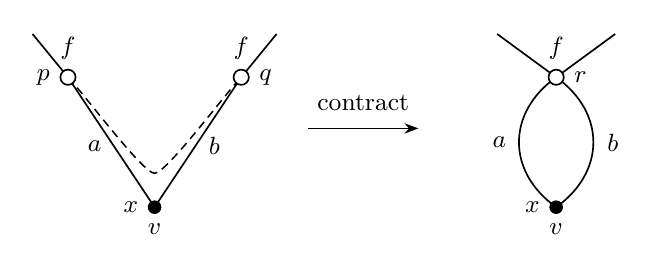
\begin{tikzpicture}[
    x=1cm, y=1cm, font=\small,
    merge white/.style={circle, draw, fill=white, line width=.6pt,
      minimum size=5.5pt, inner sep=0pt},
    merge black/.style={circle, draw, fill=black,
      minimum size=4.5pt, inner sep=0pt},
    merge edge/.style={line width=.6pt},
    merge auxiliary/.style={densely dashed, line width=.55pt}
  ]
    \begin{scope}
      \coordinate (merge-before-p-position) at (-1.1,1.65);
      \coordinate (merge-before-q-position) at (1.1,1.65);
      \coordinate (merge-before-x-position) at (0,0);
      \draw[merge edge]
        (-1.55,2.2) -- (merge-before-p-position)
        -- (merge-before-x-position) -- (merge-before-q-position)
        -- (1.55,2.2);
      \draw[merge auxiliary]
        (merge-before-p-position)
        .. controls (-.92,1.47) and (-.15,.43) .. (0,.43)
        .. controls (.15,.43) and (.92,1.47) ..
        (merge-before-q-position);
      \node[merge white, label=above:{$f$}, label=left:{$p$}]
        (merge-before-p) at (merge-before-p-position) {};
      \node[merge white, label=above:{$f$}, label=right:{$q$}]
        (merge-before-q) at (merge-before-q-position) {};
      \node[merge black, label=below:{$v$}, label=left:{$x$}]
        (merge-before-x) at (merge-before-x-position) {};
      \node at (-.76,.78) {$a$};
      \node at (.76,.78) {$b$};
    \end{scope}

    \draw[-{Stealth[length=5pt]}, line width=.6pt]
      (1.95,1) -- node[above=3pt] {contract} (3.35,1);

    \begin{scope}[xshift=5.1cm]
      \coordinate (merge-after-r-position) at (0,1.65);
      \coordinate (merge-after-x-position) at (0,0);
      \draw[merge edge]
        (-.75,2.2) -- (merge-after-r-position) -- (.75,2.2);
      \draw[merge edge]
        (merge-after-x-position)
        .. controls (-.63,.45) and (-.63,1.2) ..
        (merge-after-r-position);
      \draw[merge edge]
        (merge-after-x-position)
        .. controls (.63,.45) and (.63,1.2) ..
        (merge-after-r-position);
      \node[merge white, label=above:{$f$}, label=right:{$r$}]
        (merge-after-r) at (merge-after-r-position) {};
      \node[merge black, label=below:{$v$}, label=left:{$x$}]
        (merge-after-x) at (merge-after-x-position) {};
      \node at (-.72,.82) {$a$};
      \node at (.72,.82) {$b$};
    \end{scope}
  \end{tikzpicture}
  \caption{The white vertices $p,q$, both labelled $f$, merge to $r$
    along the dashed auxiliary arc in the empty sector between their
    consecutive edges at the black vertex $x$, labelled $v$.
    The edges of weights $a,b$ remain distinct parallel edges.}
  \label{fig:merge}
\end{figure}


\emph{Degrees, faces, and Euler's formula.}
An ordinary white vertex cannot have degree one, since its incident
weight would be nonzero.  A black vertex cannot have degree one
either, since the maps $\iota_{vi}$ are injective.  If a black vertex
had degree two, its two white neighbors would have distinct labels
by the preceding claim.  Its zero balance would then equate two
nonzero vectors in distinct one-dimensional subspaces of $K_v^0$,
which is impossible.  Consequently every black degree is at least
three, and every white degree is at least two except possibly the
exceptional degree, which is at least one.

Consider the facial boundary walks of this connected plane graph,
counting edge sides with multiplicity.  At a turn through a vertex
of degree at least two, the entering and leaving edges are distinct
and consecutive in its rotation.  Their opposite endpoints have
different labels.  Thus the image of the boundary walk in the
incidence graph has no immediate backtracking at that turn.  This
also applies to the cyclic closing turn of the walk.  Bridges cause
no difficulty: their two sides are counted separately, and a facial
walk reverses immediately along an edge only at a degree-one vertex.
There is at most one such vertex, the exceptional white vertex, and
it belongs to just one face.

It follows that all but at most one face have boundary walks whose
images are nonempty closed walks without immediate backtracking in
the incidence graph.  Such a walk contains a cycle, so each of these
faces has length at least $12$.  Write $n_{\rm b},n_{\rm w},n_{\rm f}$
for the numbers of black vertices, white vertices, and faces, and
$E$ for the number of edges.  The degree bounds and the total of
$2E$ edge sides give
\[
  n_{\rm b}\le\frac E3,\qquad
  n_{\rm w}\le\frac{E+1}{2},\qquad
  n_{\rm f}\le\frac E6+1.
\]
Therefore
\[
  n_{\rm b}+n_{\rm w}+n_{\rm f}
  \le E+\frac32<E+2,
\]
contrary to Euler's formula for a connected plane graph.  The
assumed word equality is impossible, and every $\theta_v$ is
injective.
\end{proof}

We henceforth identify $K_v^0$ with its image $K_v\le N$, and identify
$L_f^0$ with the subgroup $L_f\le N$ given by $c\mapsto s_{f,c}$,
with $0$ mapped to the identity.  The latter is injective by choosing
any point incident to $f$ and applying Lemma~\ref{lem:embedding}.
The shared generators identify this same subgroup inside every
$K_v$ with $v\in f$.  In particular, $|K_v|=\ell^2$, $|L_f|=\ell$,
and the incident subgroups $L_f$ partition $K_v$ outside the
identity.  No assertion about intersections between other local
subgroups is needed.


\section{From subgroup averages to the scalar defect}
\label{sec:packing}

The embedded groups now allow legitimate subgroup averages. We first obtain a rectangular identity, then pack its intermediate coordinates into square matrices, and finally encode those matrices as scalar elements of a group algebra. The strict size inequality will detect the reverse defect after packing.

\subsection{Subgroup averages and a rectangular identity}

We prove Theorem~\ref{thm:criterion} using the group $N$ and subgroups
$K_v,L_f\le N$ supplied by Lemma~\ref{lem:embedding}. We retain the
coordinates on $K_v$ transported from $K_v^0=\F_\ell^2$. Fix an
ordering of $V$, and use it for all matrix indices indexed by $V$.
For $v\in V$ put
\begin{equation}
\label{eq:local-average}
P_v=\kappa^{-1}\sum_{u\in K_v}u\in K[N].
\end{equation}
The integer $\kappa$ is invertible in $K$, since $\ell$ is odd. For each
$w\in K_v$ there are exactly $\kappa$ pairs $(u,u')\in K_v^2$ with
$uu'=w$, so $P_v^2=P_v$.

At a fixed $v$, the subgroups $L_f$ for $f\ni v$ run through all the
one-dimensional subspaces of the additive group $K_v$. Their nonidentity
elements partition $K_v\setminus\{1\}$. Consequently
\begin{equation}
\label{eq:subgroup-decomposition}
\sum_{u\in K_v}u
=1+\sum_{f\ni v}\left(\sum_{u\in L_f}u-1\right).
\end{equation}
This equality is internal to $K_v$; no assertion about intersections
between different $K_v$ is needed.

Write $W_v=x_vx_v^{\mathsf T}$. Define matrices over $K[N]$ by
\begin{equation}
\label{eq:rectangular-definitions}
U\in\Mat_{m\times t}(K[N]),\qquad
T\in\Mat_{t\times m}(K[N]),\qquad
U_{-,v}=-\kappa x_vP_v,\quad
T_{v,-}=P_vx_v^{\mathsf T},
\end{equation}
and set $P=\diag_{v\in V}(P_v)$. Since the entries of each $x_v$
belong to the coefficient field, they commute with all group-algebra
elements. Idempotence gives $UP=U$ and $PT=T$. Moreover,
\begin{align*}
UT
&=-\kappa\sum_{v\in V}W_vP_v^2
 =-\sum_{v\in V}W_v\sum_{u\in K_v}u\\
&=-\sum_{v\in V}W_v
 -\sum_{f\in\mathcal F}
   \left(\sum_{v\in f}W_v\right)
   \left(\sum_{u\in L_f}u-1\right)
 =I_m,
\end{align*}
where we used Equations~\eqref{eq:subgroup-decomposition} and
\eqref{eq:criterion-pairing}. We have proved
\begin{equation}
\label{eq:rectangular-identities}
UP=U,\qquad PT=T,\qquad UT=I_m.
\end{equation}

\subsection{A group extension implementing character twists}

Equation~\eqref{eq:rectangular-identities} gives the forward identity,
but the factors are rectangular. We next arrange enough orthogonal
character idempotents to place their $t$ intermediate coordinates into
$m$ slots. The extension will implement the necessary changes of character
by conjugation while preserving the original subgroup algebra.

Let $z$ generate a cyclic group of order $\ell$, and put
$H=N\times\langle z\rangle$. Choose $v_*\in V$ and put $K_*=K_{v_*}$.
For every $v\in V$ let $\phi_v:K_v\longrightarrow K_*$ be the
isomorphism taking each element to the element with identical
$\F_\ell^2$ coordinates. There are exactly $\kappa$ linear forms
$K_*\longrightarrow\F_\ell$. By Equation~\eqref{eq:criterion-size},
we may assign to each $v\in V$ a slot $s(v)\in\{1,\ldots,m\}$ and a
linear form $\alpha_v:K_*\longrightarrow\F_\ell$ so that the pairs
$(s(v),\alpha_v)$ are distinct. In particular, the forms assigned within
any one slot are distinct.

We use a multiple HNN extension~\cite[Theorem~II]{HNN1949}, verifying
the required base-group embedding directly. Adjoin to $H$ generators
$\tau_v$, $v\in V$, with relations
\begin{equation}
\label{eq:twisted-conjugation}
\tau_v(uz^r)\tau_v^{-1}
 =\phi_v(u)z^{r+\alpha_v(\phi_v(u))}
\qquad(u\in K_v,\ r\in\mathbb Z/\ell).
\end{equation}
Denote the resulting group by $L$. Exponents in $\F_\ell$ are
interpreted in $\mathbb Z/\ell$. For each $v$, the specified map
\[
\psi_v:K_v\times\langle z\rangle\longrightarrow
K_*\times\langle z\rangle,
\qquad
uz^r\longmapsto\phi_v(u)z^{r+\alpha_v(\phi_v(u))},
\]
is a group isomorphism. Its inverse takes $wz^r$ to
$\phi_v^{-1}(w)z^{r-\alpha_v(w)}$.

We verify directly that $H$ embeds in $L$. Let $H$ act on itself by left
multiplication. Restricted to either the domain or the image of
$\psi_v$, this is a disjoint union of regular actions of a subgroup of
order $\ell^3$. These two collections of orbits have the same
cardinality. Indeed, if $H$ is finite, both have $|H|/\ell^3$ orbits;
if $H$ is infinite, both have countably infinitely many, since $H$ is
countable and the subgroups are finite. Pair these orbits and choose
representatives $h_i,k_i$ so that they are respectively
$(K_v\times\langle z\rangle)h_i$ and
$(K_*\times\langle z\rangle)k_i$. The bijection
\[
F_v(ah_i)=\psi_v(a)k_i
\qquad(a\in K_v\times\langle z\rangle)
\]
of the set $H$ conjugates left multiplication by $a$ to left
multiplication by $\psi_v(a)$. Assign $F_v$ to $\tau_v$ for each $v$.
These assignments, together with the left regular action of $H$, satisfy
all the relations defining $L$: no defining relation couples two distinct
stable letters, so overlapping associated subgroups impose no additional
compatibility condition on the independently chosen $F_v$. They therefore give a permutation
representation of $L$ whose restriction to $H$ is faithful. This proves
the required embedding. In particular, $K[H]$ embeds in $K[L]$.

Taking $u=1$ in Equation~\eqref{eq:twisted-conjugation} shows that every
$\tau_v$ centralizes $z$. Since $z$ is already central in $H$, it is
central in $L$. Define
\begin{equation}
\label{eq:central-character-idempotent}
e=\ell^{-1}\sum_{r=0}^{\ell-1}\zeta^{-r}z^r\in K[L].
\end{equation}
This is a nonzero central idempotent and satisfies $ez=\zeta e$.
For completeness, in the convolution square each coefficient of $z^a$
is $\ell^{-2}\ell\zeta^{-a}$, which proves $e^2=e$; reindexing the
sum proves $ez=\zeta e$. The identity coefficient is $\ell^{-1}\ne0$
because $\langle z\rangle$ remains embedded.

For a linear form $\alpha:K_*\longrightarrow\F_\ell$, put
\begin{equation}
\label{eq:local-character-idempotent}
Q_\alpha=\kappa^{-1}\sum_{u\in K_*}\zeta^{\alpha(u)}u.
\end{equation}
Using additive notation for the coordinates of $K_*$, the coefficient
of $w$ in $Q_\alpha Q_\beta$ is
\[
\kappa^{-2}\zeta^{\beta(w)}
\sum_{u\in K_*}\zeta^{\alpha(u)-\beta(u)}.
\]
If $\alpha=\beta$, the inner sum is $\kappa$. Otherwise choose $u_0$
with $\zeta^{\alpha(u_0)-\beta(u_0)}\ne1$. Translating the summation
variable by $u_0$ multiplies the sum by this scalar while leaving it
unchanged, so the sum is zero. Thus
\begin{equation}
\label{eq:character-products}
Q_\alpha Q_\beta=
\begin{cases}
Q_\alpha,&\alpha=\beta,\\
0,&\alpha\ne\beta.
\end{cases}
\end{equation}
The conjugation relations and $ez^r=\zeta^re$ now give
\begin{equation}
\label{eq:twisted-projection}
\tau_v eP_v\tau_v^{-1}
=\kappa^{-1}\sum_{u\in K_v}
 e\phi_v(u)z^{\alpha_v(\phi_v(u))}
=eQ_{\alpha_v}.
\end{equation}

\subsection{Packing into square matrices}

The orthogonality in Equation~\eqref{eq:character-products} now lets
different coordinates share a slot without cross terms. The following
matrices implement the assignment of each coordinate $v$ to its slot
$s(v)$.

Define $C\in\Mat_{m\times t}(K[L])$ and
$J_0\in\Mat_{t\times m}(K[L])$ by
\begin{equation}
\label{eq:packing-matrices}
C_{s,v}=
\begin{cases}
\tau_veP_v,&s=s(v),\\
0,&s\ne s(v),
\end{cases}
\qquad
(J_0)_{v,s}=
\begin{cases}
eP_v\tau_v^{-1},&s=s(v),\\
0,&s\ne s(v).
\end{cases}
\end{equation}
We claim that
\begin{equation}
\label{eq:packing-identity}
J_0C=eP.
\end{equation}
The diagonal entry indexed by $v$ is $eP_v$. If $v\ne w$ have different
slots, the corresponding entry is zero. If they have the same slot,
Equation~\eqref{eq:twisted-projection} rewrites that entry as
\[
eP_v\tau_v^{-1}\tau_weP_w
=\tau_v^{-1}eQ_{\alpha_v}eQ_{\alpha_w}\tau_w=0,
\]
because $\alpha_v\ne\alpha_w$. This proves the claim.

Set
\begin{equation}
\label{eq:square-elements}
a_{\mathrm{mat}}=UJ_0+(1-e)I_m,
\qquad
b_{\mathrm{mat}}=CT+(1-e)I_m.
\end{equation}
Every entry of $C$ and $J_0$ contains the central factor $e$.
Consequently the cross terms with $1-e$ vanish, and
Equations~\eqref{eq:rectangular-identities} and
\eqref{eq:packing-identity} imply
\begin{equation}
\label{eq:square-forward-product}
a_{\mathrm{mat}}b_{\mathrm{mat}}
=U(eP)T+(1-e)I_m
=eI_m+(1-e)I_m=I_m.
\end{equation}

\subsection{Detecting the reverse defect}

Put $\Delta=b_{\mathrm{mat}}a_{\mathrm{mat}}-I_m$. We detect its
nonvanishing by multiplying on the left by $J_0$ and on the right by
$C$. This brings the calculation back from $K[L]$ to its embedded
subgroup algebra $K[H]$, where a scalar specialization is available.
Direct multiplication
gives $\Delta=CTUJ_0-eI_m$, and hence
\begin{equation}
\label{eq:reverse-sandwich}
J_0\Delta C=(eP)TU(eP)-eP=e(TU-P).
\end{equation}
In the last equality the order of multiplication is essential:
$(eP)TU(eP)=e(PT)(UP)=eTU$. The right-hand side of
Equation~\eqref{eq:reverse-sandwich} already belongs to
$\Mat_t(K[H])$.

There is a $K$-algebra homomorphism
\begin{equation}
\label{eq:subgroup-specialization}
\varepsilon:K[H]\longrightarrow K,
\qquad
\varepsilon(nz^r)=\zeta^r\quad(n\in N).
\end{equation}
It is well-defined because $H=N\times\langle z\rangle$.
It sends $e$ to $1$ and each $P_v$ to $1$.
Let $X\in\Mat_{m\times t}(K)$ be the matrix with columns $x_v$.
Since the characteristic is two and $\kappa$ is odd,
\[
\varepsilon(U)=X,\qquad
\varepsilon(T)=X^{\mathsf T},\qquad
XX^{\mathsf T}=I_m.
\]
Thus
\begin{equation}
\label{eq:specialized-defect}
\varepsilon\bigl(e(TU-P)\bigr)=X^{\mathsf T}X-I_t.
\end{equation}
Because $t>m$, choose a nonzero $y\in\ker X$. Then
\begin{equation}
\label{eq:nonzero-witness}
\varepsilon\bigl(e(TU-P)\bigr)y=-y\ne0.
\end{equation}
One explicit choice is the first nonzero column of $I_t-X^{\mathsf T}X$:
this matrix is nonzero because $\rank(X^{\mathsf T}X)\le m<t$, and
$X(I_t-X^{\mathsf T}X)=0$. This choice uses only finite-field
arithmetic on the given vectors.

Equation~\eqref{eq:nonzero-witness} proves that $e(TU-P)$ is nonzero in
$\Mat_t(K[H])$. The embedding $K[H]\subseteq K[L]$ and
Equation~\eqref{eq:reverse-sandwich} therefore show that $\Delta\ne0$.
The homomorphism $\varepsilon$ has been applied only to elements of
$K[H]$; no extension of it to $K[L]$ is used.

\subsection{From matrices to two group-algebra elements}

The square factors give a failure of stable finiteness for $K[L]$.
To obtain scalar factors, we embed $\Mat_m(K[L])$ in an idempotent
corner of $K[L\times F]$ for a suitable finite group $F$. The identity
of this corner need not be the identity of the whole group algebra;
adding its complement to both factors will give a scalar product equal
to $1$. This is an explicit instance of the finite-factor reduction
of Dykema and Juschenko~\cite[Theorem~2.2]{DykemaJuschenko2015}.

For the finite matrix block, let
\begin{equation}
\label{eq:finite-auxiliary-group}
B=(\mathbb Z/\ell)^m,
\qquad
F=B\rtimes S_m,
\end{equation}
where $S_m$ permutes the coordinates. For $1\le i\le m$ define
\begin{equation}
\label{eq:coordinate-idempotents}
p_i=|B|^{-1}\sum_{w\in B}\zeta^{-w_i}w\in K[F].
\end{equation}
The coordinate characters are distinct. The character-sum calculation
used in Equation~\eqref{eq:character-products}, now on $B$, shows that
the $p_i$ are pairwise orthogonal idempotents. Each is nonzero, since its
identity coefficient is $|B|^{-1}$. This denominator exists because
$|B|=\ell^m$ is odd. No inverse of $|S_m|$ is required.

Let $\sigma_i\in S_m$ exchange coordinates $1$ and $i$, taking
$\sigma_1=1$. Then $\sigma_i p_1\sigma_i^{-1}=p_i$. Put
\begin{equation}
\label{eq:finite-matrix-units}
p_{ij}=\sigma_i p_1\sigma_j^{-1}\qquad(1\le i,j\le m).
\end{equation}
These elements are nonzero, being left and right translates of $p_1$,
and they satisfy $p_{ii}=p_i$ and $p_i p_{ij}p_j=p_{ij}$.
For $j\ne k$ the latter identity and $p_jp_k=0$ give
$p_{ij}p_{kr}=0$. For $j=k$, direct cancellation gives
$p_{ij}p_{jr}=\sigma_i p_1^2\sigma_r^{-1}=p_{ir}$. Thus
\begin{equation}
\label{eq:matrix-unit-products}
p_{ij}p_{kr}=\delta_{jk}p_{ir}.
\end{equation}
The matrix units are linearly independent over $K$: multiplying a
linear relation on the left by $p_i$ and on the right by $p_j$ isolates
its coefficient of the nonzero element $p_{ij}$.

Take
\begin{equation}
\label{eq:output-group}
G=L\times F.
\end{equation}
We regard $K[L]$ and $K[F]$ as commuting subalgebras of $K[G]$, and put
\begin{equation}
\label{eq:block-embedding}
f_{\mathrm{blk}}=\sum_{i=1}^m p_{ii},
\qquad
\Phi:\Mat_m(K[L])\longrightarrow K[G],
\qquad
\Phi(Z)=\sum_{i,j=1}^m Z_{ij}p_{ij}.
\end{equation}
Equation~\eqref{eq:matrix-unit-products} proves that $\Phi$ is
multiplicative and that $\Phi(I_m)=f_{\mathrm{blk}}$.
It is also injective. Indeed, the group basis identifies
$K[L\times F]$ with $K[L]\otimes_K K[F]$. If $\Phi(Z)=0$, expand
each entry as $Z_{ij}=\sum_{g\in L}c_{ij,g}g$. Comparing the
$L$-basis coefficient of each $g$ gives
$\sum_{i,j}c_{ij,g}p_{ij}=0$. The linear independence just proved
forces every $c_{ij,g}$ to be zero.

The required two elements are
\begin{equation}
\label{eq:output-elements}
\boxed{\begin{aligned}
a_{\mathrm{out}}
 &=1-f_{\mathrm{blk}}+
   \sum_{i,j=1}^m
   \bigl((UJ_0)_{ij}+(1-e)\delta_{ij}\bigr)p_{ij},\\
b_{\mathrm{out}}
 &=1-f_{\mathrm{blk}}+
   \sum_{i,j=1}^m
   \bigl((CT)_{ij}+(1-e)\delta_{ij}\bigr)p_{ij}.
\end{aligned}}
\end{equation}
Equivalently, these are $1-f_{\mathrm{blk}}+\Phi(a_{\mathrm{mat}})$
and $1-f_{\mathrm{blk}}+\Phi(b_{\mathrm{mat}})$, respectively.
The matrix-unit identities imply
\[
f_{\mathrm{blk}}^2=f_{\mathrm{blk}},
\qquad
f_{\mathrm{blk}}\Phi(Z)=\Phi(Z)=\Phi(Z)f_{\mathrm{blk}}.
\]
Therefore $1-f_{\mathrm{blk}}$ annihilates every image of $\Phi$ on
both sides. It follows from Equation~\eqref{eq:square-forward-product}
that
\[
a_{\mathrm{out}}b_{\mathrm{out}}
=1-f_{\mathrm{blk}}+\Phi(I_m)=1,
\]
whereas
\begin{equation}
\label{eq:output-defect}
b_{\mathrm{out}}a_{\mathrm{out}}-1=\Phi(\Delta)\ne0
\end{equation}
by injectivity. Only the identity action of $f_{\mathrm{blk}}$ on the
image of $\Phi$ is needed for these computations.

\subsection{Finite presentation and the retained odd torsion}
\label{sec:finite-presentation}

All sums in Equation~\eqref{eq:output-elements} are finite, as are the
sums defining their entries. We now verify the remaining assertions about
the group $G$ by tracking its presentation through the construction.

Let $N=\langle\mathcal S_N\mid\mathcal R_N\rangle$ be the finite
presentation from Section~\ref{sec:criterion}, with the generators
$s_{f,c}$ and the local zero-sum relators of length at most three. With
$[x,y]=xyx^{-1}y^{-1}$, the direct product with the cyclic group has the
finite presentation
\[
H=\left\langle\mathcal S_N,z\ \middle|\;
\mathcal R_N,\ z^\ell,\ [z,s]\ (s\in\mathcal S_N)\right\rangle.
\]
Every element of $K_v$ and $K_*$ in
Equation~\eqref{eq:twisted-conjugation} has a representative given by
its local generator, or by the empty word for the identity. Using those
representatives, that equation adds $|V|$ stable letters and at most
$|V|\ell^3$ relators to the displayed presentation of $H$: its indices
are $v\in V$, $u\in K_v$, and $r\in\mathbb Z/\ell$. Hence $L$ is
finitely presented. The permutation action used above proves that the
base group embeds; its choices do not add generators or relators.

The group $F=(\mathbb Z/\ell)^m\rtimes S_m$ is finite, so its finite
multiplication table gives a finite presentation. A presentation of
$G=L\times F$ consists of finite presentations of the two factors on
disjoint generator sets, together with the commutators of every generator
of $L$ with every generator of $F$. This adds only finitely many relators,
and therefore $G$ is finitely presented. Finally, the embeddings already
proved give
\[
K_v\le N\le H\le L\le G.
\]
Since $K_v$ is the additive group of $\F_\ell^2$, its nonidentity
elements have order $\ell$. The output group therefore contains the
asserted odd-order torsion. This completes the proof of
Theorem~\ref{thm:criterion}.

The construction proves a failure of direct finiteness for a group
algebra by exhibiting its two elements. In particular, the last step
does not infer stable finiteness from direct finiteness for an arbitrary
ring: it uses the explicit finite group $F$ and the injective map
$\Phi$.

\section{A regular hypergraph of affine lines}\label{sec:hypergraph}

The algebraic criterion is now complete. Its remaining input is a line
system satisfying Proposition~\ref{prop:pairing}: full lines avoiding a
set of holes of controlled size, with exact regularity and incidence
girth at least $12$.
Starting from line partitions gives regularity, but simply deleting the
lines through a hole would lower the degree of other points as well.
We instead arrange the lines through each hole in planar bundles that
can be replaced by parallel lines missing the hole. Each replacement
preserves every other point's degree. We choose the holes to make these
replacements compatible, then use random three-dimensional slabs to
exclude the remaining short incidence cycles.

Let $q=2^h$ and let $\ell$ be the least prime congruent to $-1$ modulo
$q^{100}$. The residue $q^{100}-1$ is coprime to $q^{100}$. Linnik's theorem~\cite{Linnik1944} gives absolute constants $c,L>0$ such that
this prime exists and $\ell\le c q^{100L}$; see, for example,
\cite[Theorem~1.1]{Xylouris2011}.  Set
\begin{equation}\label{eq:hypergraph-parameters}
 D=\ell+1,\qquad s=\lfloor\log_qD\rfloor,\qquad
 b=s+20,\qquad n=10b,\qquad N_{\rm pt}=q^n.
\end{equation}
Thus $q^{100}\mid D$, $s\ge100$, and
\begin{equation}\label{eq:hypergraph-growth}
 q^s\le D<q^{s+1}.
\end{equation}
Moreover, $s$ is bounded independently of $h$: indeed,
$D\le(c+1)q^{100L}$ implies
$s\le100L+\log_2(c+1)$.  In this section all asymptotic statements refer
to $h\to\infty$.  Constants implicit in $O(\cdot)$ may depend on a
fixed upper bound for $s$, but not on $h$, the field enumeration,
or the indices of the objects being counted. Thus $s$ and $n$ may vary
with $h$, but the estimates below use fixed upper bounds for them.

The divisibility $q\mid D$ permits bundles of $q$ directions. The lower
bound $s\ge100$ makes the hole-selection estimates small, and the slack
in $b=s+20$ controls the later event weights. The factor ten in $n=10b$
permits ten-wise independent subspaces in the construction below. Each
step of a short polygon will involve at most two of these subspaces,
so their directness will cover polygons with at most five steps.

Let $Q$ be a field of order $q$, with any enumeration
$(a_0,\ldots,a_{q-1})$, and put $\mathcal A=Q^n$.  Define
\begin{equation}\label{eq:hypergraph-lower-set}
 d_0=(q-2)/2,\qquad
 S=\left\{(a_{i_1},\ldots,a_{i_n}):
                  i_1+\cdots+i_n\le d_0\right\}.
\end{equation}
An affine line always means a full translate of a one-dimensional
$Q$-subspace, and consequently contains exactly $q$ points.

\begin{theorem}\label{thm:hypergraph}
For all sufficiently large $h$, for every $Q$ and enumeration as above,
there are a set $O\subset S$ and a set $\mathcal F$ of affine lines
contained in $V=\mathcal A\setminus O$ such that
\begin{equation}\label{eq:hypergraph-hole-size}
 \frac{2N_{\rm pt}}{D^2}\le |O|\le\frac{7N_{\rm pt}}{D^2},
\end{equation}
every point of $V$ lies on exactly $D$ members of $\mathcal F$, and
the bipartite incidence graph of $V$ and $\mathcal F$ has girth at
least $12$.
\end{theorem}

\subsection{Direction spaces and the local trade}

Divide an index set of size $D$ into $D/q$ bundles of size $q$.
Write $\rho(j)$ for the bundle containing an index $j$.

\begin{lemma}\label{lem:hypergraph-direction-spaces}
There are two-dimensional subspaces $W_r\subset\mathcal A$, one per
bundle, and $(b-1)$-dimensional subspaces $E_j\subset\mathcal A$,
one per index, such that any at most ten distinct members of this list
have direct sum.  Choose a direction $e_r$ in each $W_r$, and assign
its other $q$ directions bijectively to the indices in that bundle,
calling them $d_j$.  Then $U_j=d_j\oplus E_j$ has dimension $b$, and
\begin{equation}\label{eq:hypergraph-intersections}
 U_j\cap U_{j'}=0\quad(j\ne j'),\qquad
 U_j\cap e_r=0,\qquad
 U_j\cap W_r=
 \begin{cases}d_j,&r=\rho(j),\\0,&r\ne\rho(j).
 \end{cases}
\end{equation}
\end{lemma}

\begin{proof}
Let $Q'/Q$ be an extension of degree $b$, and identify the $Q$-space
$\mathcal A$ with $(Q')^{10}$.  For distinct $\xi\in Q'$, the vectors
$(1,\xi,\ldots,\xi^9)$ have the property that any at most ten are
linearly independent over $Q'$: the first $k$ coordinates of $k$ such
vectors form an invertible Vandermonde matrix.  There are enough
parameters because
$D+D/q<q^{s+2}\le q^b$.  Give each $W_r$ and $E_j$ its own parameter,
and choose it, of the prescribed $Q$-dimension, inside the corresponding
one-dimensional $Q'$-space.  These choices have the required directness.

To verify the intersections, any equality involving $U_j$ and $U_{j'}$
first has zero $E_j$- and $E_{j'}$-components.  Its remaining components
belong either to independent $W$-spaces or to distinct directions in
one $W$-space.  In both cases they vanish.  The other assertions follow
the same way; within $W_{\rho(j)}$ the directions $d_j$ and $e_{\rho(j)}$
are distinct.
\end{proof}

\Needspace{10\baselineskip}
Fix these spaces for the rest of the construction. The eventual
preliminary partition indexed by $j$ will use varying directions in
$U_j$, with $o+d_j$ its line through a hole $o$; the spaces $E_j$
provide the other directions. If these $q$ axes are present for a
bundle $r$, then inside $o+W_r$ they can be replaced by the $q-1$
lines parallel to $e_r$ other than $o+e_r$. Each point off $o+e_r$
loses and gains one incidence, the hole loses $q$, and the remaining
points of $o+e_r$ are unaffected. Figure~\ref{fig:hypergraph-trade}
illustrates this local count. The hole restrictions and slab construction
below will supply these axes and make all the trades simultaneously
possible.
\begin{figure}[htbp]
\centering
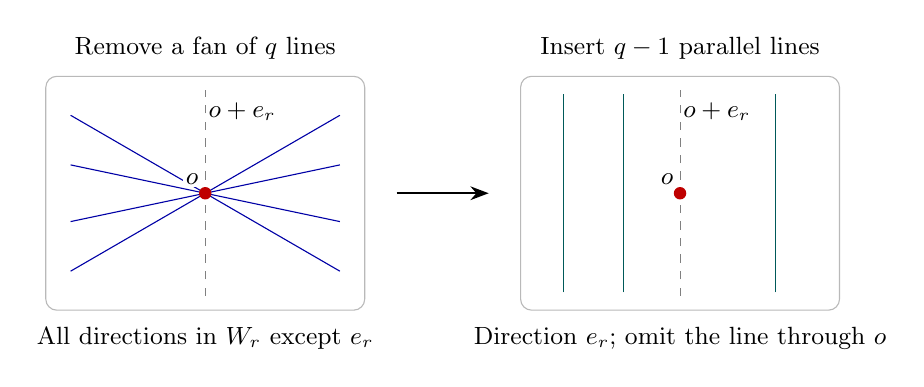
\begin{tikzpicture}[>=Stealth,scale=.9,
  every node/.style={font=\small}]
 \begin{scope}[shift={(-3.35,0)}]
  \draw[rounded corners,gray!55] (-2.25,-1.65) rectangle (2.25,1.65);
  \node at (0,2.05) {Remove a fan of $q$ lines};
  \draw[gray,dashed] (0,-1.45)--(0,1.45);
  \draw[blue!65!black] (-1.9,-1.1)--(1.9,1.1);
  \draw[blue!65!black] (-1.9,-.4)--(1.9,.4);
  \draw[blue!65!black] (-1.9,.4)--(1.9,-.4);
  \draw[blue!65!black] (-1.9,1.1)--(1.9,-1.1);
  \fill[red!75!black] (0,0) circle (2.5pt);
  \node[fill=white,inner sep=1pt,above left] at (-.05,.08) {$o$};
  \node[fill=white,inner sep=1pt,above right] at (0,.98) {$o+e_r$};
  \node at (0,-2.05) {All directions in $W_r$ except $e_r$};
 \end{scope}
 \draw[->,thick] (-.65,0)--(.65,0);
 \begin{scope}[shift={(3.35,0)}]
  \draw[rounded corners,gray!55] (-2.25,-1.65) rectangle (2.25,1.65);
  \node at (0,2.05) {Insert $q-1$ parallel lines};
  \draw[gray,dashed] (0,-1.45)--(0,1.45);
  \draw[teal!70!black] (-1.65,-1.4)--(-1.65,1.4);
  \draw[teal!70!black] (-.8,-1.4)--(-.8,1.4);
  \draw[teal!70!black] (1.35,-1.4)--(1.35,1.4);
  \fill[red!75!black] (0,0) circle (2.5pt);
  \node[fill=white,inner sep=1pt,above left] at (-.05,.08) {$o$};
  \node[fill=white,inner sep=1pt,above right] at (0,.98) {$o+e_r$};
  \node at (0,-2.05) {Direction $e_r$; omit the line through $o$};
 \end{scope}
\end{tikzpicture}
\caption{Schematic of the trade inside $o+W_r$.
Every point off $o+e_r$ loses and gains one incidence;
$o$ loses $q$ incidences, and other points of $o+e_r$ are unaffected.
The strokes illustrate line families, not a real-plane realization
of finite-field incidences.}
\label{fig:hypergraph-trade}
\end{figure}


\subsection{Choosing compatible holes}

The replacement lines are parallel within a bundle, but lines from two
bundles could form a rectangle. We prevent this while choosing the holes.
An \emph{exceptional rectangle} has corners
$x,x+u,x+u+v,x+v$, where $0\ne u\in e_r$, $0\ne v\in e_{r'}$,
and $r\ne r'$.  For each of its four side lines, a \emph{witness}
is a point off that line but in the translate of $W_r$ or $W_{r'}$
containing it, according to the side's direction.
If that side is produced by a trade, its hole is such a witness.

\Needspace{13\baselineskip}
\begin{lemma}\label{lem:hypergraph-holes}
For all sufficiently large $h$, there is $O\subset S$ satisfying
Equation~\eqref{eq:hypergraph-hole-size} and the following properties.
\begin{enumerate}[label=\textup{(\roman*)}]
 \item Every translate of every $W_r$ contains at most one point of $O$.
 \item For every $j$, every coset $C$ of $U_j$, and every $r$,
       $|O\cap(C+W_r)|\le100$.
 \item No exceptional rectangle has four distinct witnesses in $O$,
       one for each of its four side lines.
\end{enumerate}
\end{lemma}

\begin{proof}
Write $M=N_{\rm pt}/D^2$.  Since $d_0<q$, counting nonnegative index
tuples gives $|S|=\binom{d_0+n}{n}$.  For large $h$, $d_0\ge q/3$,
so
\[
 |S|\ge \frac{q^n}{3^n n!}\ge c_S N_{\rm pt}
\]
with a constant $c_S>0$ independent of $h$, because $n$ is bounded.
Choose each point of $S$ independently with probability
$\theta=5M/|S|$.  For large $h$ this is at most $1$, and
$\theta=O(D^{-2})$.  If $X$ is the chosen set, then
$\mathbb E|X|=5M$ and $\operatorname{Var}(|X|)\le5M$.
Also $M>q^{n-2s-2}=q^{8s+198}\to\infty$.
Chebyshev's inequality therefore gives
\begin{equation}\label{eq:hypergraph-initial-holes}
 \Pr(4M\le |X|\le6M)=1-o(1).
\end{equation}

There are at most $D^2N_{\rm pt}$ triples $(j,r,C)$, and every
$C+W_r$ has at most $q^{b+2}$ points.  Repeated affine spaces in
this count only cause overcounting.  A union bound over choices of
$100$ selected points bounds the probability that any such space
contains more than $100$ points of $X$ by
\[
 D^2N_{\rm pt}(\theta q^{b+2})^{100}
 =O\left(q^{2s+2+n+100(b+2-2s)}\right)
 =O\left(q^{2402-88s}\right)=o(1).
\]

Mark every selected point belonging to a pair of distinct selected
points in one translate of some $W_r$.  Also mark every selected
point belonging to a tuple of four distinct selected witnesses for
an exceptional rectangle.  The expected number of collision pairs
is at most
$N_{\rm pt}(D/q)q^2\theta^2$.  There are at most
$N_{\rm pt}(D/q)^2(q-1)^2\le N_{\rm pt}D^2$
choices of rectangle data, and at most $q^8$ witness tuples per
rectangle.  Each distinct tuple is selected with probability at most
$\theta^4$; tuples containing a point outside $S$ have probability zero.
Thus the number $Z$ of marked points satisfies
\[
 \frac{\mathbb EZ}{M}
 \le \frac{2N_{\rm pt}(D/q)q^2\theta^2
             +4N_{\rm pt}D^2q^8\theta^4}{M}
 =O\left(\frac qD+\frac{q^8}{D^4}\right)=o(1).
\]
Markov's inequality gives $Z\le M$ with probability $1-o(1)$.
Choose an outcome satisfying this bound, Equation~\eqref{eq:hypergraph-initial-holes},
and the occupancy bound, and delete all marked points.  The remaining
set $O$ has $3M\le |O|\le6M$, hence the required bounds.  Deletion
preserves the occupancy bound and eliminates every obstruction in
\textup{(i)} and \textup{(iii)}.
\end{proof}

Fix such an $O$.  Put
\[
 T_r=\bigcup_{o\in O}(o+W_r).
\]
The \emph{replacement lines of label $R_r$} are all the lines of
direction $e_r$ in each $o+W_r$, except $o+e_r$ itself.

\begin{lemma}\label{lem:hypergraph-replacement-lines}
The replacement lines avoid $O$ and are pairwise disjoint within
each label $R_r$.  No exceptional rectangle has all four side lines
among these replacement lines.
\end{lemma}

\begin{proof}
Property~\textup{(i)} of Lemma~\ref{lem:hypergraph-holes} says that
different holes lie in disjoint translates of a fixed $W_r$.
Within one such plane the replacement lines are parallel and omit
its unique hole.  This proves the first assertions.

If a rectangle used four replacement lines, each side would have
its corresponding hole as a witness.  These four witnesses must
be distinct.  Opposite sides of direction $e_r$ lie in $W_r$-cosets
separated by a nonzero vector in $e_{r'}$, which lies outside $W_r$.
Their planes are therefore disjoint.  The planes of two adjacent
sides intersect exactly at their shared corner, because
$W_r\cap W_{r'}=0$.  This corner is on both side lines, so neither
off-line witness can equal it.  The resulting four distinct witnesses
contradict property~\textup{(iii)} of Lemma~\ref{lem:hypergraph-holes}.
\end{proof}

\subsection{Random slabs and short polygons}

The holes and the replacement lines are now fixed. It remains to
partition the rest of the space into lines without introducing short
polygons. We first choose the slabs in which those lines will lie,
excluding a finite list of events that would allow such polygons;
the line partitions themselves are constructed only afterward.

Independently for each index $j$ and each coset $C$ of $U_j$, choose
a uniformly random two-dimensional subspace $P_{j,C}\subset E_j$.
The translates of $d_j\oplus P_{j,C}$ partition $C$ into
three-dimensional affine \emph{slabs}.  For $u\in U_j$, write
$u^{(E_j)}$ for its
$E_j$-component.  A fixed nonzero vector of $E_j$ belongs to $P_{j,C}$
with probability
\begin{equation}\label{eq:hypergraph-inclusion-probability}
 p_* = \frac{q^2-1}{q^{b-1}-1}\le 2q^{3-b}.
\end{equation}
Indeed, linear automorphisms of $E_j$ act transitively on its nonzero
vectors, and every two-dimensional subspace contains $q^2-1$ of them.

We define a finite list of bad events before selecting any lines
inside the slabs.  First, for each pair of holes in a coset $C$ of
$U_j$, declare it bad if they occupy the same slab.  Their difference
has nonzero $E_j$-component: otherwise it would lie in
$d_j\subset W_{\rho(j)}$, contrary to
Lemma~\ref{lem:hypergraph-holes}\textup{(i)}.  This event is exactly
the inclusion of that component in $P_{j,C}$ and has probability $p_*$.

The other events concern closed labelled sequences of $k$ nonzero
steps, $k\in\{3,4,5\}$, in $\mathcal A$.  The allowed step types are
\begin{align*}
 G_j &: \quad u\in U_j,\quad u^{(E_j)}\ne0;\\
 R_r &: \quad u\in e_r\setminus\{0\},
               \quad\hbox{both endpoints belong to }T_r.
\end{align*}
We call $G_j$ steps \emph{generic} and $R_r$ steps \emph{replacement}
steps; a replacement step vector will also be called exceptional.
An $R_r$ step need not lie on a replacement line: its endpoint condition
only requires membership in $T_r$, which every actual replacement line
satisfies. This deliberately enlarges the list of possible polygons.
Require at least one $G$ step and distinct labels at cyclically
adjacent steps.  Repeated vertices are allowed, so this list can
only be larger than the list of simple polygons that will matter
for girth.  For each such sequence, declare it bad if every $G_j$
step has $u^{(E_j)}\in P_{j,C}$, where $C$ is the $U_j$-coset
containing that step.  All point, label, and step choices are finite,
so the complete event list is finite.

The three hole conditions now have separate roles. Condition~\textup{(i)}
separates the replacement planes within each bundle and makes each
hole-pair event test a nonzero $E_j$-component. Condition~\textup{(ii)}
controls the hole contributions to the event counts for a fixed
$P_{j,C}$. Condition~\textup{(iii)} has already excluded rectangles
formed entirely from replacement lines.

\Needspace{8\baselineskip}
\begin{lemma}\label{lem:hypergraph-polygons}
Every candidate sequence with a generic step has one of the following
forms.
\begin{enumerate}[label=\textup{(\roman*)}]
 \item A rectangle alternating $G_j,R_r$, with opposite vectors paired.
 \item A rectangle alternating distinct $G_j,G_{j'}$, with opposite
       vectors paired.
 \item A pentagon containing two $G_j$ steps, two $G_{j'}$ steps,
       and one $R_r$ step, where $\rho(j)=\rho(j')=r$.
\end{enumerate}
If $g$ is the number of distinct generic labels, its bad event uses
$2g$ distinct random variables and has probability $p_*^{2g}$.
In case~\textup{(iii)}, the exceptional vector and one vector of each
generic label determine the other two vectors, once their order is fixed.
\end{lemma}

\begin{proof}
Before classifying the sequence, observe that each step involves
at most two members of the list of $W$- and $E$-spaces.  Thus at most
$2k\le10$ distinct spaces occur, and their directness is available
from Lemma~\ref{lem:hypergraph-direction-spaces}.
Closure forces the sum of the $E_j$-components to be zero for each
generic label.  Each such label therefore occurs at least twice.
Cyclic non-adjacency in a sequence of at most five steps allows
any label at most twice.  Consequently $g$ is $1$ or $2$, and each
generic label occurs exactly twice.

If $g=1$, the direction $d_j$ and the distinct occurring directions
$e_r$ are linearly independent.  In its own bundle this uses just the
two distinct directions $d_j,e_{\rho(j)}$; other bundles contribute
independent $W$-spaces.  Every exceptional label must therefore occur
twice as well.  Only case~\textup{(i)} is possible, and closure gives
the claimed opposite vectors.

If $g=2$ and $k=4$, the labels must alternate, and
$U_j\cap U_{j'}=0$ forces the opposite vectors to pair.
If $k=5$, there is one exceptional step, of label $R_r$.
Its nonzero $e_r$-component must be canceled by the $W$-components
of the generic steps.  Neither zero contribution nor a contribution
from just one of the directions $d_j,d_{j'}$ can cancel it, since
each such direction differs from $e_r$.  Thus both generic labels belong
to bundle $r$, giving case~\textup{(iii)}.  After choosing the exceptional
vector and one vector of each generic label, closure prescribes the
sum of the remaining vector in $U_j$ and the remaining vector in
$U_{j'}$.  Their direct sum makes these vectors unique.

Finally, between the two occurrences of a generic label $G_j$ there
is, in one cyclic direction, exactly one intervening step.  That
step has a different label and a nonzero vector outside $U_j$, by
Equation~\eqref{eq:hypergraph-intersections}.  The two occurrences
therefore belong to different $U_j$-cosets: if the first starts at $x$
with vector $u\in U_j$ and the intervening vector is $v\notin U_j$,
the second starts at $x+u+v\notin x+U_j$. Variables from different
generic labels are also distinct.  All $2g$ variables are consequently
independent, and Equation~\eqref{eq:hypergraph-inclusion-probability}
gives the asserted event probability.
\end{proof}

\subsection{Avoiding the slab events}

The classification controls the probability of each polygon event. To
avoid all events simultaneously, we must also control how many of them
use any one slab variable. We bound the sum of their probabilities at
a fixed $P_{j,C}$; the local lemma will apply once this bound is at most
$1/16$.

\begin{lemma}\label{lem:hypergraph-event-bounds}
Let $\mu$ be the largest, over all variables $P_{j,C}$, of the sum
of probabilities of bad events using that variable.  Then
$\mu=O(q^{-7})$, uniformly in the variable, and every event uses
at most four variables.
\end{lemma}

\begin{proof}
The assertion about four variables follows from
Lemma~\ref{lem:hypergraph-polygons}, with one variable for a hole-pair
event.  Fix $P_{j,C}$.  There are at most $100$ holes in $C$, since
$C\subset C+W_r$ for any $r$.  Hole pairs therefore contribute at most
$100^2p_*$.

For a polygon using this variable, cyclically rotate so that one of
its $G_j$ steps starts the sequence.  Rotations and orders of at most
five labels introduce only an absolute constant factor in all the
following counts.  For a generic rectangle choose the other label
($\le D$ choices), the sequence's initial point in $C$ ($q^b$ choices), and
one vector of each label ($\le q^{2b}$ choices).  Closure determines
the other two vectors.  The contribution is therefore
$O(Dq^{3b}p_*^4)$.

For a mixed rectangle $G_j,R_r$, both endpoints of the initial
generic step belong to $C\cap T_r$.  A hole $o$ can contribute to
this intersection only if $o\in C+W_r$, so there are at most $100$
such holes.  Each intersection $C\cap(o+W_r)$, when nonempty, is
a coset of $U_j\cap W_r$.  It has $q$ points if $r=\rho(j)$ and one
point otherwise. Thus $C\cap T_r$ has at most $100q$ points in the
first case and at most $100$ in the second. Choose the two endpoints,
and then choose the
exceptional vector in $e_r$ in at most $q$ ways.  Summing over the
$D/q$ bundles gives at most
\[
 O\left(100^2\left(q^3+\frac Dq\,q\right)\right)
   =O\bigl(100^2(q^3+D)\bigr)
\]
mixed rectangles, and hence a contribution
$O(100^2(q^3+D)p_*^2)$.  This is an upper bound even when some
selected endpoints or vectors fail the candidate conditions.

For a pentagon the other generic label is in bundle $\rho(j)$,
giving at most $q$ choices.  Choose the sequence's initial point in $C$,
one vector of each generic label, and the exceptional vector.
There are at most $q^{b+2b+1}$ choices after the label is chosen.
Lemma~\ref{lem:hypergraph-polygons} determines the remaining vectors,
so the contribution is $O(q^{3b+2}p_*^4)$.

In total,
\begin{align*}
 \mu
 &\le 100^2p_*+
 O\left(Dq^{3b}p_*^4+(D+q^3)p_*^2+q^{3b+2}p_*^4\right)\\
 &=O\left(q^{-s-17}+q^{-7}+q^{-s-33}
                      +q^{-2s-31}+q^{-s-6}\right)
 =O(q^{-7}),
\end{align*}
using $b=s+20$, Equation~\eqref{eq:hypergraph-growth}, and
Equation~\eqref{eq:hypergraph-inclusion-probability}.  The constants
in these event counts are absolute; in particular the bound is uniform.
\end{proof}

The following is a special case of the asymmetric Lov\'asz local
lemma; we include the classical conditional-probability proof.
For the origins see Erd\H{o}s and Lov\'asz~\cite{ErdosLovasz1975};
for the product-form condition used below see
\cite[Theorem~1.1]{MoserTardos2009}. No resampling algorithm is needed.

\begin{lemma}\label{lem:hypergraph-local-lemma}
Let a finite collection of events be determined by independent
random variables, with each event assigned a nonempty set of at most
four variables that determine it.
If the sum of event probabilities at every variable is at most
$1/16$, there is positive probability that no event occurs.
\end{lemma}

\begin{proof}
Connect two events when their assigned sets share a variable.  An event
is independent of all its non-neighbors jointly.  Set $x_A=2\Pr(A)$.
Since each event has a nonempty assigned set, $0\le x_A\le1/8<1$,
and for every event
\[
 \sum_{B\text{ neighbor of }A}x_B\le 2\cdot4\cdot\frac1{16}
 =\frac12.
\]
It follows that
\begin{equation}\label{eq:hypergraph-local-lemma-condition}
 \Pr(A)\le x_A\prod_{B\text{ neighbor of }A}(1-x_B),
\end{equation}
because the product is at least $1-\sum_Bx_B\ge1/2$.

We prove inductively that
\[
 \Pr\left(A\,\middle|\,\bigcap_{B\in\mathcal S}B^c\right)\le x_A
\]
whenever $\mathcal S$ is a sublist excluding $A$, and that all
conditioning events in this assertion have positive probability.
The empty sublist follows from
Equation~\eqref{eq:hypergraph-local-lemma-condition}.
At each induction step, positivity for a sublist follows by exposing
its events in order and using the smaller conditional bounds and
$x_B<1$.  For the bound, split $\mathcal S$ into neighbors and
non-neighbors of $A$.  Let $B_0$ be avoidance of the non-neighbors
and $D_0$ avoidance of the neighbors.  Independence gives
$\Pr(A\mid B_0)=\Pr(A)$, and
\[
 \Pr(A\mid B_0\cap D_0)
 \le \frac{\Pr(A)}{\Pr(D_0\mid B_0)}
 \le \frac{\Pr(A)}
 {\prod_{B\in\mathcal S,\ B\text{ neighbor of }A}(1-x_B)}
 \le x_A.
\]
The middle bound uses the smaller conditional bounds successively;
the last uses Equation~\eqref{eq:hypergraph-local-lemma-condition}.
The same successive conditioning for the full finite event list
gives positive probability of avoiding all events.
\end{proof}

By Lemmas~\ref{lem:hypergraph-event-bounds} and
\ref{lem:hypergraph-local-lemma}, for all sufficiently large $h$ we
can fix the spaces $P_{j,C}$ so that every slab contains at most one
hole and none of the candidate polygon events occurs.

\subsection{Line partitions, the local trade, and girth}

The slab choices have excluded every candidate short polygon with a
generic step, but no line partition has yet been specified. We now
partition each slab, perform the trades that remove the holes, and
check that every possible short incidence cycle is one of the
excluded polygons.

\begin{lemma}\label{lem:hypergraph-slab-partition}
Let a three-dimensional affine space have direction $P\oplus d$,
where $\dim_QP=2$ and $\dim_Qd=1$.  If it has no designated point,
it has a line partition whose directions project nontrivially to $P$.
If it has a designated point $o$, it has a line partition containing
$o+d$, with every other line's direction projecting nontrivially to $P$.
\end{lemma}

\begin{proof}
In the first case use parallel lines of any fixed nonzero direction
in $P$.  In the second choose $0\ne\delta\in d$ and a $Q$-linear
operator $J$ on $P$ with no eigenvector over $Q$.  Identify $P$ with
the $Q$-space of a quadratic field extension of $Q$, and let $J$ be
multiplication by an element $\eta$ outside $Q$.  An equation
$\eta x=\lambda x$ with $x\ne0$ and $\lambda\in Q$ would imply
$\eta=\lambda$, so this operator has the required property.
Besides $o+d$, use the lines
\begin{equation}\label{eq:hypergraph-slab-lines}
 \left\{o+x+\gamma(Jx)\delta:
                   x\in P,\ \gamma(x)=1\right\},
 \qquad 0\ne\gamma\in\operatorname{Hom}_Q(P,Q).
\end{equation}
The set $\gamma(x)=1$ is an affine line in $P$.  Its displayed lift
is injective, with direction projecting onto the nonzero line
$\ker\gamma$, so it is an affine line with the required direction.
For each $x\ne0$, the vectors $x,Jx$ form a basis of $P$.
For every $c\in Q$ there is consequently exactly one functional
with $\gamma(x)=1$ and $\gamma(Jx)=c$, and it is nonzero.
Thus the $q^2-1$ lines in Equation~\eqref{eq:hypergraph-slab-lines}
partition the $q^3-q$ points off $o+d$.  The axis $o+d$ supplies the
remaining $q$ points.
\end{proof}

For each $j$, apply Lemma~\ref{lem:hypergraph-slab-partition}
separately in every slab of every coset of $U_j$, using its unique
hole as the designated point when present.  This gives a preliminary
line partition of all of $\mathcal A$ for each $j$.  The line through
a hole $o$ in partition $j$ is $o+d_j$.  These hole axes are the only
lines whose directions have zero $E_j$-component.  Every other line
has a nonzero $E_j$-component in its direction, lying in the
corresponding $P_{j,C}$.

\begin{lemma}\label{lem:hypergraph-trade}
For every hole $o$ and bundle $r$, remove the $q$ lines $o+d_j$ with
$\rho(j)=r$, and insert the $q-1$ replacement lines of label $R_r$
in $o+W_r$.  After all these operations, the resulting set
$\mathcal F$ consists of lines in $V$, and every point of $V$ has
degree $D$.  The surviving lines of each preliminary partition are
pairwise disjoint, as are the replacement lines within each label.
There are no duplicate lines across different labels.
\end{lemma}

\begin{proof}
Within $o+W_r$, the removed fan uses every direction except $e_r$.
Each point off $o+e_r$ lies on exactly one removed line and exactly
one inserted line.  The hole $o$ loses $q$ incidences and gains none;
other points of $o+e_r$ lose and gain none.  Thus every non-hole point
has zero net change in degree in each trade.

No removal is requested twice.  Two holes using the same line of
one preliminary partition would be in the same slab, which was
excluded.  Lines from distinct preliminary partitions have directions
in distinct $U_j$'s with zero intersection, so cannot coincide.
Inserted lines of a given label are distinct by
Lemma~\ref{lem:hypergraph-replacement-lines}.  Lines of different
labels cannot coincide either: their direction spaces are distinct
$U_j$'s or $e_r$'s with pairwise zero intersections, by
Lemma~\ref{lem:hypergraph-direction-spaces}.
Hence the pointwise degree changes genuinely add when all trades
are performed, even if planes from different bundles overlap.
Initially every point has one incidence in each of the $D$ partitions.
Each hole loses all $D$ of its incidences, and every non-hole retains
degree $D$.  All inserted lines avoid the holes, and all preliminary
lines through a hole were removed.  Finally, disjointness within a
surviving preliminary label is inherited from its partition, and
disjointness within a replacement label was proved in
Lemma~\ref{lem:hypergraph-replacement-lines}.
\end{proof}

The pointwise incidence changes are summarized in
Figure~\ref{fig:hypergraph-trade}.

\begin{proof}[Proof of Theorem~\ref{thm:hypergraph}]
Use the holes from Lemma~\ref{lem:hypergraph-holes}, the successful
slab choices, and the line family from Lemma~\ref{lem:hypergraph-trade}.
The size and degree assertions have been proved.  Label surviving
preliminary lines from partition $j$ by $G_j$, and replacement lines
by their labels $R_r$.

Two distinct affine lines have at most one common point, so a cycle
of length less than $12$ in the incidence graph would give a polygon
of $k=3,4$, or $5$ nonzero steps along its successive lines.
Consecutive labels, including the last and first, are different
because lines of one label are disjoint.  If there is a generic step,
this polygon is one of the candidate sequences used above.  Each
generic step's $E_j$-component lies in its slab direction $P_{j,C}$,
so the corresponding bad event would occur, a contradiction.

If all steps have replacement labels, the distinct occurring $e_r$
directions are independent: at most five $W_r$'s occur.
Closure forces every label to occur at least twice, while cyclic
non-adjacency allows at most twice.  The only possibility is a
four-step alternating rectangle, with opposite vectors paired.
This is forbidden by Lemma~\ref{lem:hypergraph-replacement-lines}.
Thus the incidence girth is at least $12$.
\end{proof}

This supplies the full-line system, exact degree, and girth required by
Proposition~\ref{prop:pairing}. That proposition uses the same holes to
produce the two matrix pairings and the size inequalities for
Theorem~\ref{thm:criterion}. Section~\ref{sec:prescription} now makes the
choices by finite enumeration.

\section{A terminating prescription for the witnesses}
\label{sec:prescription}

We now fix every choice in the preceding construction. The purpose of the prescription is to define one field, one group, and two finite sums without relying on an unspecified successful random choice.

\subsection{Finite search for the incidence data}

Order binary coefficient vectors lexicographically, with $0<1$; for a polynomial of fixed degree use the list of coefficients in increasing degree order. For each integer $h\ge2$, perform the following finite computations.
\begin{enumerate}[label=\textup{(\arabic*)}]
\item Put $q=2^h$, and let $\ell$ be the least prime congruent to $-1$ modulo $q^{100}$. Test successive integers in that class for primality. Linnik's theorem guarantees that this search terminates. Define $D=\ell+1$, $s=\lfloor\log_qD\rfloor$, $b=s+20$, and $n=10b$ as in Section~\ref{sec:hypergraph}.
\item Let $g$ be the lexicographically first monic irreducible polynomial over $\F_2$ of degree $h(\ell-1)$, and put
\begin{equation}
\label{eq:exact-field}
K=\F_2[Z]/(g(Z)).
\end{equation}
Order $K$ by the coefficient vectors of its unique representatives of degree less than $h(\ell-1)$, padded by zeros. Irreducible polynomials of this degree exist, and irreducibility is a finite test.
\item Take the subfield
\[
Q=\{x\in K:x^q=x\},
\]
with its induced order. It has $q$ elements since $h$ divides $h(\ell-1)$. Let $\zeta$ be the first element of $K$ of multiplicative order $\ell$. Such an element exists: Fermat's little theorem gives $\ell\mid 2^{\ell-1}-1$, so $\ell$ divides $|K^\times|=2^{h(\ell-1)}-1$, and $K^\times$ is cyclic.
\item Form $\mathcal A=Q^n$ in lexicographic order and the index simplex $S$ of Section~\ref{sec:pairing}. Order subsets of a finite ordered set by their indicator vectors, with $0<1$. In particular this orders affine lines as subsets of $\mathcal A$, families of lines as subsets of the ordered line set, and pairs $(O,\mathcal F)$ lexicographically. Test every pair with $O\subset S$ and $\mathcal F$ a family of full affine $Q$-lines for the following conditions:
\begin{enumerate}[label=\textup{(\alph*)}]
\item $2q^n/D^2\le |O|\le7q^n/D^2$;
\item every line of $\mathcal F$ is contained in $\mathcal A\setminus O$;
\item every point of $\mathcal A\setminus O$ lies on exactly $D$ lines of $\mathcal F$;
\item the incidence graph has no cycle of length less than $12$.
\end{enumerate}
\end{enumerate}
Start with $h=2$. For a fixed $h$, step~\textup{(4)} tests only finite sets and a finite graph. Stop at the first successful pair; if every pair fails, increase $h$ by one and repeat. This selects the least successful $h$ and then the first successful pair in its prescribed order. Theorem~\ref{thm:hypergraph} guarantees success for every sufficiently large $h$, uniformly in the enumeration of $Q$, so the outer search terminates. The search enumerates the required incidence data directly, not the auxiliary random choices used to prove their existence. The auxiliary extension field in that proof is only a model for a $Q$-vector space; it is not required to embed in $K$.

Fix these data and write $m=|O|$, $t=|V|$, where $V=\mathcal A\setminus O$. The indicator polynomials $f_o$ and vectors $x_v$ are the unique ones from Proposition~\ref{prop:pairing}; their coefficients may be computed by finite-field linear algebra. We use the induced orders on $O$, $V$, and $\mathcal F$.

\subsection{Local groups, the presentation, and the two sums}

At each point $v$, use the standard coordinate copy $K_v^0=(\F_\ell^2,+)$, and for each line $f$ use $L_f^0=(\F_\ell,+)$. Order $\F_\ell$ by the residues $0,\ldots,\ell-1$ and $\F_\ell^2$ lexicographically. Order its one-dimensional subspaces as subsets. Match them in order to the $D=\ell+1$ incident lines at $v$, and define $\iota_{vf}$ by sending $1\in L_f^0$ to the first nonzero vector of the assigned direction. These maps specify the group $N$ in Lemma~\ref{lem:embedding} without any further choices.

Choose $v_*$ to be the first point of $V$. The isomorphism $\phi_v:K_v\to K_{v_*}$ preserves the standard coordinates transported from the embedded copies. Order linear forms on $\F_\ell^2$ by their coefficient pairs. Assign the points of $V$, in order, to the first $t$ pairs
\[
(s,\alpha),\qquad 1\le s\le m,\quad \alpha\in(\F_\ell^2)^*,
\]
in lexicographic order. Proposition~\ref{prop:pairing} gives $t\le m\ell^2$, so there are enough pairs. This fixes every slot and every character in the construction of Theorem~\ref{thm:criterion}.

For the finite presentation of $N$, use the local zero-sum relators of length at most three, as justified in Section~\ref{sec:criterion}. Section~\ref{sec:packing} then defines $H=N\times\langle z\rangle$, the conjugation extension $L$, the finite group $F=(\mathbb Z/\ell)^m\rtimes S_m$, and finally $G=L\times F$; Section~\ref{sec:finite-presentation} gives the resulting finite presentation. The regular-permutation action used to prove that $H$ embeds in $L$ is an embedding certificate; a choice of such permutations is not part of the definition of the group.

With this group fixed, the formulas in Section~\ref{sec:packing} give $e,P,U,T,C,J_0$, the two square matrices $a_{\rm mat},b_{\rm mat}$, and the matrix units $p_{ij}$. The two required finite expressions are
\begin{equation}
\label{eq:exact-outputs}
\begin{split}
a_{\mathrm{out}}&=1-\sum_{i=1}^m p_{ii}
 +\sum_{i,j=1}^m(a_{\rm mat})_{ij}p_{ij},\\
b_{\mathrm{out}}&=1-\sum_{i=1}^m p_{ii}
 +\sum_{i,j=1}^m(b_{\rm mat})_{ij}p_{ij}.
\end{split}
\end{equation}
Coefficients from $K[L]$ and matrix units from $K[F]$ are viewed in the two factors of $K[G]$. The displayed expressions, together with the preceding formulas, involve only finitely many group words and field coefficients. They define finite sums whether or not distinct displayed words represent the same group element; no word-equality oracle is used to normalize them.

\begin{proof}[Proof of Theorem~\ref{thm:main}]
The finite search terminates by Theorem~\ref{thm:hypergraph}. Its output satisfies Proposition~\ref{prop:pairing}, and hence every hypothesis of Theorem~\ref{thm:criterion}. That theorem proves the two product assertions for \eqref{eq:exact-outputs}, supplies a finite presentation of this group $G$, and retains an embedded element of order $\ell$. In particular the nonvanishing of the reverse-product defect follows by specializing the right-hand side of Equation~\eqref{eq:reverse-sandwich}, which lies in $\Mat_t(K[H])$, to a nonzero matrix over $K$; it does not depend on an unproved inequality between group words. The prime $\ell$ is odd, and the field in \eqref{eq:exact-field} is finite of characteristic two.
\end{proof}

\subsection{Scope of the construction}

The construction uses torsion explicitly. The embedded subgroups of orders $\ell$, $\ell^2$, and $\ell^3$ have odd order, so every denominator in their averages is invertible in $K$. In the finite auxiliary group we invert only $|(\mathbb Z/\ell)^m|$, never $|S_m|$. Characteristic two makes the regular degree $\ell+1$ vanish as a scalar, allowing the simultaneous line and total pairing identities of Proposition~\ref{prop:pairing}. No assertion about group algebras of torsion-free groups is needed.

For comparison, if $G_0$ is finite, then $K_0[G_0]$ is finite dimensional over every field $K_0$, even when the characteristic divides $|G_0|$. Left multiplication is a faithful representation of this algebra. In finite dimension, $L_aL_b=I$ implies $L_bL_a=I$, and hence $ab=1$ implies $ba=1$. Thus the group in Theorem~\ref{thm:main} is necessarily infinite.

Finally, for any group and any two finite group-algebra sums, the union of their supports generates a finitely generated subgroup. Its group algebra embeds in the original one, so both product assertions already hold or fail in that subgroup algebra. Finite generation is therefore automatic for a direct-finiteness counterexample after passing to the support subgroup. The stronger finite-presentation conclusion for the particular group $G$ here comes from the presentation argument in Section~\ref{sec:finite-presentation}; it does not follow merely from finite generation of the support subgroup.

\section{An injective nonsurjective cellular automaton}
\label{sec:cellular}

The scalar elements constructed in Section~\ref{sec:prescription} now
give a cellular automaton over the finite alphabet $K$. We prove the
standard transfer explicitly, in the right-neighbor convention used
in the introduction; compare\ \cite[Section~1]{ElekSzabo2004}.
The proof applies to all configurations, not just finitely supported
ones, and identifies the image by finite local equations.

\subsection{The group algebra acting on all configurations}

For this subsection, let $K$ be any field and $G$ any group, with
identity $1_G$. For $c=\sum_{u\in G}c_u u\in K[G]$, put
$\supp(c)=\{u\in G:c_u\ne0\}$. Multiplication in $K[G]$ is
\[
  (cd)_w=\sum_{uv=w}c_ud_v.
\]
Every sum has only finitely many nonzero terms. Define a $K$-linear map
$T_c:K^G\to K^G$ by
\begin{equation}
\label{eq:ca-operator}
  (T_cx)(g)=\sum_{u\in G}c_u x(gu).
\end{equation}
This sum is finite even when $x$ has infinite support. If $K$ is
finite, it is a cellular automaton with memory $\supp(c)$.

\begin{lemma}
\label{lem:ca-representation}
For every field $K$ and group $G$, the assignment $c\mapsto T_c$ is
a faithful unital $K$-algebra homomorphism from $K[G]$ to the algebra
of $K$-linear endomorphisms of $K^G$, with composition as multiplication.
In particular,
\begin{equation}
\label{eq:ca-composition}
  T_c\circ T_d=T_{cd},\qquad T_1=\id_{K^G}.
\end{equation}
\end{lemma}

\begin{proof}
Linearity in $c$ and the identity $T_1=\id_{K^G}$ follow directly
from Equation~\eqref{eq:ca-operator}. For $x\in K^G$ and $g\in G$,
\begin{align*}
 (T_c(T_dx))(g)
 &=\sum_{u\in G}c_u\sum_{v\in G}d_vx(guv)\\
 &=\sum_{w\in G}\left(\sum_{uv=w}c_ud_v\right)x(gw)
 =(T_{cd}x)(g).
\end{align*}
All sums being regrouped are finite. In particular, the product is
$cd$, not $dc$, for this right-neighbor convention.

For $h\in G$, let $\delta_h\in K^G$ take value $1_K$ at $h$ and
zero elsewhere. Then
\begin{equation}
\label{eq:ca-coefficient}
  (T_c\delta_h)(1_G)=c_h.
\end{equation}
Thus $T_c=0$ implies that every coefficient $c_h$ is zero, proving
faithfulness.
\end{proof}

\subsection{The local rule and its image}

\begin{proposition}
\label{prop:ca-transfer}
Let $K$ be a finite field, $G$ a group, and $a,b\in K[G]$ satisfy
$ab=1$. Put $M=\supp(b)$ and define
\begin{equation}
\label{eq:ca-rule}
  \phi:K^M\longrightarrow K,
  \qquad \phi(p)=\sum_{u\in M}b_up(u).
\end{equation}
The cellular automaton $\tau=T_b$ is injective, and
\begin{equation}
\label{eq:ca-image}
  \im(\tau)=\{y\in K^G:T_{ba}y=y\}.
\end{equation}
If $ba\ne1$, every $h\in G$ with $(ba-1)_h\ne0$ gives a
configuration $\delta_h\notin\im(\tau)$; hence $\tau$ is not
surjective.
\end{proposition}

\begin{proof}
The support of $b$ is finite, so Equation~\eqref{eq:ca-rule} is a
single finite-memory local rule, used at every $g\in G$. The alphabet
$K$ is finite and nonempty. Lemma~\ref{lem:ca-representation} gives
\begin{equation}
\label{eq:ca-leftinverse}
  T_a\circ\tau=T_{ab}=T_1=\id_{K^G}.
\end{equation}
Applying $T_a$ to $\tau(x)=\tau(x')$ yields $x=x'$ for arbitrary
$x,x'\in K^G$.

If $y=\tau(x)=T_bx$, then
\[
  T_{ba}y=T_bT_aT_bx=T_bx=y,
\]
by Equation~\eqref{eq:ca-leftinverse}. Conversely, if $T_{ba}y=y$,
then $y=T_b(T_ay)$ lies in the image of $\tau$. This proves
Equation~\eqref{eq:ca-image}.

If $(ba-1)_h\ne0$, Equation~\eqref{eq:ca-coefficient} gives
\[
  \bigl(T_{ba}\delta_h-\delta_h\bigr)(1_G)
  =\bigl(T_{ba-1}\delta_h\bigr)(1_G)
  =(ba-1)_h\ne0.
\]
Therefore $\delta_h$ is not fixed by $T_{ba}$, and
Equation~\eqref{eq:ca-image} excludes it from the image. This
calculation also covers $h=1_G$, when $\delta_h(1_G)=1_K$ rather
than zero.
\end{proof}

Equation~\eqref{eq:ca-image} describes the image by the uniform
finite local equations
\[
  \sum_{u\in\supp(ba-1)}(ba-1)_u\,y(gu)=0
  \qquad(g\in G).
\]
Thus the missing configuration has no preimage even among infinitely
supported functions. No restriction to finitely supported
configurations has entered the argument.

The memory need not be minimal. If a finite expression for $b$ is
$b=\sum_{j=1}^r\lambda_j u_j$, with $\lambda_j\in K$ and
$u_j\in G$ and with repetitions allowed, take
$M'=\{u_j:1\le j\le r\}$ and
$\phi'(p)=\sum_{j=1}^r\lambda_j p(u_j)$. Repeated group elements
automatically combine to give the same operator $T_b$. Consequently,
the finite word expressions of Equation~\eqref{eq:exact-outputs}
specify the local rule without an algorithm deciding which displayed
words represent the same group element.

\begin{corollary}
\label{cor:nonsurjunctive}
For the field $K$, group $G$, and outputs of
Theorem~\ref{thm:main}, the cellular automaton
$T_{b_{\mathrm{out}}}:K^G\to K^G$ is injective and not surjective.
Its image is the fixed set of $T_{b_{\mathrm{out}}a_{\mathrm{out}}}$.
In particular, $G$ is not surjunctive.
\end{corollary}

\begin{proof}
Apply Proposition~\ref{prop:ca-transfer} to
$a=a_{\mathrm{out}}$ and $b=b_{\mathrm{out}}$. Their product
relations are proved in Theorem~\ref{thm:main}, and the nonzero
reverse-product defect has a nonzero coefficient in the ordinary
group algebra.
\end{proof}

Characteristic two is used to construct the algebraic witnesses,
not in Proposition~\ref{prop:ca-transfer}. Finiteness of the field
supplies the finite alphabet, and the scalar form of the witnesses
makes that alphabet $K$ itself rather than a vector space over $K$.
The existence of a nonzero defect coefficient is certified
algebraically; no practical execution of the finite search or
normalization of group words is asserted.

\subsection{Transport to a group of type \texorpdfstring{$F_\infty$}{F infinity}}

A group has type $F_\infty$ if it admits a classifying CW complex with
finitely many cells in every dimension. The finite presentation of $G$
allows a further consequence: a separate embedding theorem transports
the same scalar counterexample to an overgroup of type $F_\infty$.

\begin{corollary}
\label{cor:finfty-counterexample}
For the finite characteristic-two field $K$ of Theorem~\ref{thm:main},
there are a group $U$ of type $F_\infty$ and scalar elements
$A,B\in K[U]$ such that $AB=1$ and $BA\ne1$.
The group $U$ is nonsofic and nonsurjunctive.
\end{corollary}

\begin{proof}
The group $G$ in Theorem~\ref{thm:main} is finitely presented.
The companion embedding theorem~\cite[Theorem~1.1]{UniversalFinftyCompanion}
therefore gives an injection $i:G\hookrightarrow U$ into a group of
type $F_\infty$. Extending $i$ linearly over the same field $K$ gives a
unital algebra injection $i_*:K[G]\hookrightarrow K[U]$: distinct group
basis elements remain distinct. Set $A=i_*(a_{\mathrm{out}})$ and
$B=i_*(b_{\mathrm{out}})$. Then
\[
 AB=1,\qquad
 BA-1=i_*(b_{\mathrm{out}}a_{\mathrm{out}}-1)\ne0.
\]
If $U$ were sofic, Elek--Szab\'o's theorem
\cite[Corollary~4.7]{ElekSzabo2004} would make $K[U]$ stably finite,
contradicting these scalar identities. Proposition~\ref{prop:ca-transfer},
applied to $U,K,A,B$, makes $T_B:K^U\to K^U$ an injective nonsurjective
cellular automaton over the finite alphabet $K$, with left inverse
$T_A$ in the same right-neighbor convention. Hence $U$ is nonsurjunctive.
\end{proof}

\bibliographystyle{alphaurl}
\bibliography{references}
\end{document}
